\documentclass[9pt]{beamer}
\usepackage{fontspec}
\usepackage[english,bulgarian]{babel}
\usepackage{xcolor}
\usepackage{amsmath}
\usepackage{mathtools} 

\defaultfontfeatures{Ligatures=TeX}
\newfontfamily\cyrillicfont{Comfortaa-Regular}
\newfontfamily\cyrillicfonttt{Comfortaa-Regular}
\newfontfamily\fontcomic[NFSSFamily=roboto]{Roboto}
\setsansfont{Comfortaa-Regular}
\usefonttheme[onlymath]{serif}

\definecolor{mygreen}{rgb}{0.3333, 0.4196, 0.1843}
\definecolor{mypink}{rgb}{0.858, 0.188, 0.478}

\graphicspath{ {./resources/} }

\newcommand{\Q}[1]{\left[#1\right]}
\newcommand{\B}[1]{\left(#1\right)}


\usetheme{metropolis}
\begin{document}
    \section{Разпознаване на емоции в сигнали от реч и ЕЕГ}
    \begin{frame}{В началото}
        \begin{itemize}
            \item ... бе Словото
            \pause 
            \item Експлицитен и имплицитен канал при общуване
            \pause 
            \item Прозодия (ритъм, интонация, ударение)
        \end{itemize}
        \pause 
        \begin{center}
            \includegraphics[width=\textwidth]{meaning.png}%

            \footnotesize{Попълването на вица е оставено за упражнение на читателя}
            \normalsize
        \end{center}
        \pause
        \begin{itemize}
            \item Съчетаване на първичен (ЕЕГ) и вторичен (реч) канал
        \end{itemize}        
    \end{frame}
    
    \begin{frame}{Влакче на мисълта}
        \begin{center}
        \begin{itemize}
            \setlength\itemsep{\fill}
            \item[$\triangleright$] Нулева зона (какво е емоция)
            \pause 
            \item[$\triangleright$] Сигнал от реч
            \pause 
            \item[$\triangleright$] Сигнал от ЕЕГ
            \pause 
            \item[$\triangleright$] Съчетаване на двата сигнала
            \pause 
            \item[$\triangleright$] Резултати
            \pause 
            \item[$\triangleright$] Заключение
        \end{itemize}
        \end{center}
    \end{frame}

    \section{Нулева зона (какво е емоция)}
    \begin{frame}{Нулева зона (какво е емоция)}
        \begin{itemize}
            \setlength\itemsep{\fill}
            \item Теорията на Дарвин
            \begin{itemize}
                \pause
                \item[$-$] ``Принцип на полезните навици''
                \pause
                \item[$-$] ``Принцип на противоположностите''
                \pause
                \item[$-$] ``Принцип на нервните сигнали''
            \end{itemize}
            \pause
            \item Продължението на Плутчик (1980)
        \end{itemize}
        \pause
        \begin{quote}
            \textbf{Емоцията е сложна верига от събития, която започва с някакъв стимул.} В следствие настъпва фаза на ``изпитване на емоция'' и фаза на физиологични промени. Те предизвикват целенасочено държание, което цели да премахне дразнението на стимула и да върне състоянието на еквилибриум.
        \end{quote}
    \end{frame}
    \begin{frame}{Нулева зона (какво е емоция)}
        \begin{columns}[T] % align columns
            \begin{column}{.53\textwidth}
                \begin{center}
                    \includegraphics[width=\textwidth]{plutchik}%
                \end{center}
            \end{column}%
            \hfill%
            \pause
            \begin{column}{.45\textwidth}
                \vspace{1cm}
                ${\color{mygreen}+}$ Всяка емоция може да се изрази като комбинация на основните
                
                \vspace{2cm}
                \pause
                ${\color{mypink}-}$ Осем е голямо число
            \end{column}%
        \end{columns}
    \end{frame}
    \setbeamercolor{background canvas}{bg=white}
    \begin{frame}{Нулева зона (какво е емоция)}
        \begin{itemize}
            \item VAD модела - Алберт Мейерабиан и Джеймс Ръсел (1974)
        \end{itemize}
        \pause
        \begin{center}
            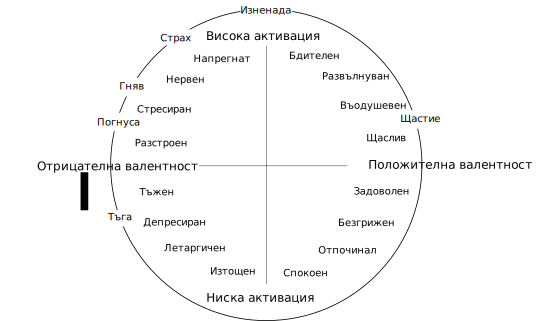
\includegraphics[width=0.8\textwidth]{valence_arousal}%
        \end{center}
        \pause
        \begin{itemize}
            \item В сигнала от реч се измерва по-лесно активацията
            \pause
            \item В сигнала от ЕЕГ се измерва по-лесно валентността
        \end{itemize}
    \end{frame}

    \begin{frame}{Нулева зона (какво е емоция)}
        \begin{columns}[T] % align columns
            \begin{column}{.38\textwidth}
                \textbf{Избрани емоции:}
                \vspace{1cm} \leavevmode \newline
                \phantom{$\bullet\ $ Гняв}
                \vspace{1cm} \leavevmode \newline
                \phantom{$\bullet\ $ Щастие}
                \vspace{1cm} \leavevmode \newline
                \phantom{$\bullet\ $ Неутрална емоция}
                \vspace{1cm} \leavevmode \newline
                \phantom{$\bullet\ $ Тъга}
            \end{column}%
            \hfill%
            \begin{column}{.60\textwidth}
                \vspace{1cm}
                \begin{center}
                    \includegraphics[width=\textwidth]{valence_arousal_empty}%
                \end{center}
            \end{column}%
        \end{columns}
    \end{frame}

    \begin{frame}{Нулева зона (какво е емоция)}
        \begin{columns}[T] % align columns
            \begin{column}{.38\textwidth}
                \textbf{Избрани емоции:}
                \vspace{1cm} \leavevmode \newline
                $\bullet\ $ Гняв
                \vspace{1cm} \leavevmode \newline
                \phantom{$\bullet\ $ Щастие}
                \vspace{1cm} \leavevmode \newline
                \phantom{$\bullet\ $ Неутрална емоция}
                \vspace{1cm} \leavevmode \newline
                \phantom{$\bullet\ $ Тъга}
            \end{column}%
            \hfill%
            \begin{column}{.60\textwidth}
                \vspace{1cm}
                \begin{center}
                    \includegraphics[width=\textwidth]{valence_arousal_a}%
                \end{center}
            \end{column}%
        \end{columns}
    \end{frame}


    \begin{frame}{Нулева зона (какво е емоция)}
        \begin{columns}[T] % align columns
            \begin{column}{.38\textwidth}
                \textbf{Избрани емоции:}
                \vspace{1cm} \leavevmode \newline
                $\bullet\ $ Гняв
                \vspace{1cm} \leavevmode \newline
                $\bullet\ $ Щастие
                \vspace{1cm} \leavevmode \newline
                \phantom{$\bullet\ $ Неутрална емоция}
                \vspace{1cm} \leavevmode \newline
                \phantom{$\bullet\ $ Тъга}
            \end{column}%
            \hfill%
            \begin{column}{.60\textwidth}
                \vspace{1cm}
                \begin{center}
                    \includegraphics[width=\textwidth]{valence_arousal_ah}%
                \end{center}
            \end{column}%
        \end{columns}
    \end{frame}

    \begin{frame}{Нулева зона (какво е емоция)}
        \begin{columns}[T] % align columns
            \begin{column}{.38\textwidth}
                \textbf{Избрани емоции:}
                \vspace{1cm} \leavevmode \newline
                $\bullet\ $ Гняв
                \vspace{1cm} \leavevmode \newline
                $\bullet\ $ Щастие
                \vspace{1cm} \leavevmode \newline
                $\bullet\ $ Неутрална емоция
                \vspace{1cm} \leavevmode \newline
                \phantom{$\bullet\ $ Тъга}
            \end{column}%
            \hfill%
            \begin{column}{.60\textwidth}
                \vspace{1cm}
                \begin{center}
                    \includegraphics[width=\textwidth]{valence_arousal_ahn}%
                \end{center}
            \end{column}%
        \end{columns}
    \end{frame}


    \begin{frame}{Нулева зона (какво е емоция)}
        \begin{columns}[T] % align columns
            \begin{column}{.38\textwidth}
                \textbf{Избрани емоции:}
                \vspace{1cm} \leavevmode \newline
                $\bullet\ $ Гняв
                \vspace{1cm} \leavevmode \newline
                $\bullet\ $ Щастие
                \vspace{1cm} \leavevmode \newline
                $\bullet\ $ Неутрална емоция
                \vspace{1cm} \leavevmode \newline
                $\bullet\ $ Тъга
            \end{column}%
            \hfill%
            \begin{column}{.60\textwidth}
                \vspace{1cm}
                \begin{center}
                    \includegraphics[width=\textwidth]{valence_arousal_ahns}%
                \end{center}
            \end{column}%
        \end{columns}
    \end{frame}

    \section{Сигнал от реч}

    \begin{frame}{Сигнал от реч - физическа обосновка}
        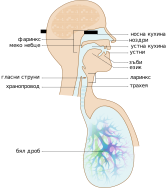
\includegraphics[width=0.48\paperwidth]{physics}%
        \hfill
        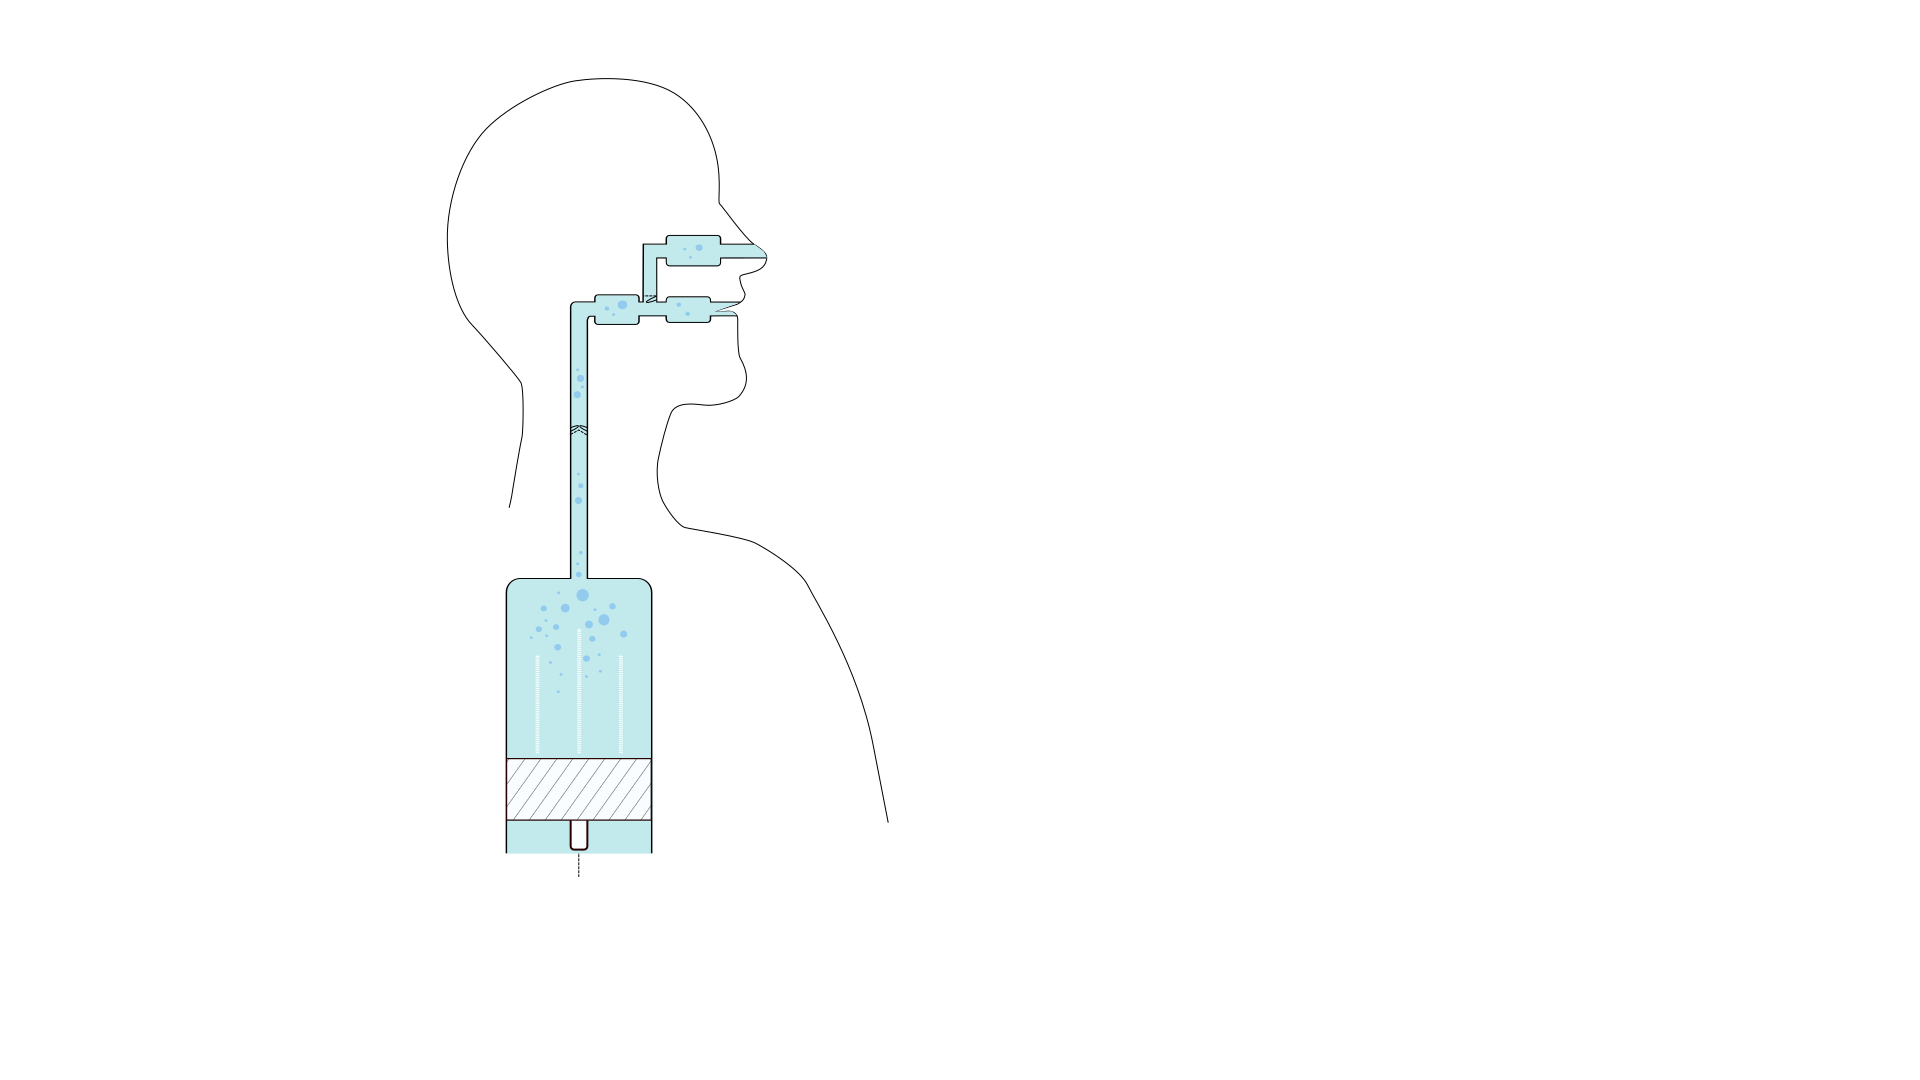
\includegraphics[width=0.28\paperwidth]{tubes}%
    \end{frame}

    \begin{frame}{Сигнал от реч - физическа обосновка}
        \centering{
            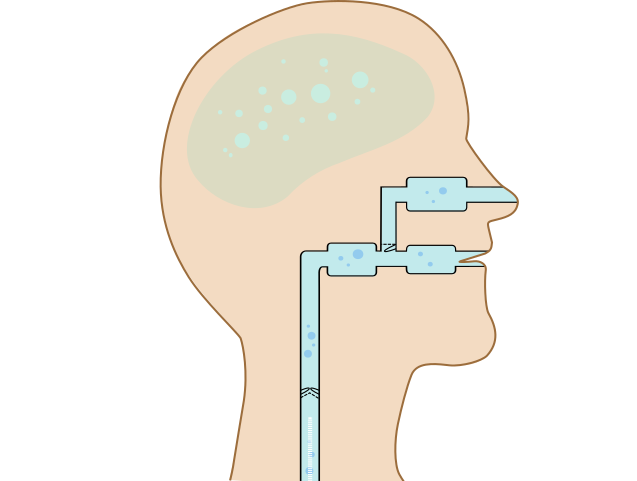
\includegraphics[height=\textheight]{glottis}%
        }
    \end{frame}

    \begin{frame}{Сигнал от реч - физическа обосновка}
    Видове звуци:
    \vspace{1cm} \leavevmode \newline
    \pause
    \begin{itemize}
        \item Озвучени - ``а''
        \pause
        \item Проходни (фрикативни) - ``с''
        \pause
        \item Преградни - ``п'' 
    \end{itemize}
    \vspace{1cm}
    \pause
    Реч \pause$\rightarrow$ думи \pause $\rightarrow$ фонеми 
    \vspace{1cm} \leavevmode \newline
    \pause
    ``Страхът стискаше гърлото, задушаваше гласа.''
    \end{frame}

    \begin{frame}{Сигнал от реч - физическа обосновка}
        \begin{itemize}
            \item Спектрални характеристики
            \pause
            \item Честотна пропускливост
        \end{itemize}
        \pause
        \centering{
            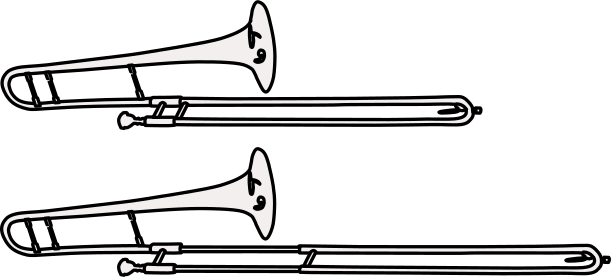
\includegraphics[width=\textwidth]{trombone}%
        }
        \pause
        \textbf{За да изследваме подлежащата емоция, трябва да изследваме спектралните свойства на статична конфигурация на вокалния тракт.}
    \end{frame}

    \begin{frame}{Сигнал от реч - модел на тръбите}
        \begin{itemize}
            \setlength\itemsep{\fill}
            \item Ще моделираме системата за производство на реч с модела на тръбите
            \pause
            \item Искаме да отделим вокалния тракт от останалите компоненти
            \pause
            \item Да разгледаме фонемата ``ъ''
            \pause
            \item Глотисът $\textbf{g}$ трепти, вокалният тракт $\textbf{v}$ филтрира сигнала, и вълната евентуално излиза и допълнително се променя от устните $\textbf{r}$ 
            \pause
            \item[$\ $] Ако  $g(t) \xleftrightarrow{\mathcal{F}\mathcal{S}} \mathcal{G}(z), v(t) \xleftrightarrow{\mathcal{F}\mathcal{S}} \mathcal{V}(z), r(t) \xleftrightarrow{\mathcal{F}\mathcal{S}} \mathcal{R}(z)$, а новият сигнал е $y$ с $y(t)=g(t)\ast v(t) \ast r(t), y(t) \xleftrightarrow{\mathcal{F}\mathcal{S}} Y(z)$, е изпълнено, че
            \pause
            \item $\mathcal{Y}(z) = \mathcal{G}(z) \mathcal{V}(z) \mathcal{R}(z)$
        \end{itemize}
    \end{frame}

    \begin{frame}{Сигнал от реч - модел на тръбите}
    \centering{
        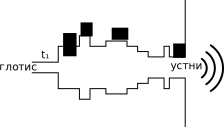
\includegraphics[width=0.7\textwidth]{vocal_tubes}%
    }
    \begin{itemize}
        \item{$c$} - скорост на звука в еластична среда
        \item{$\rho$} - плътност на въздуха в тръбите
        \item{$A$} - лицето на напречното сечение в тръба (константа)
        \item{$u = u(x, t)$} - е обемната скорост на позиция $x$ в момента $t$
        \item{$p = p(x, t)$} - е звуковото налягане
    \end{itemize}
    \end{frame}
    
    \begin{frame}[t]{Сигнал от реч - модел на тръбите}
        \begin{columns}[T]
            \begin{column}{0.48\textwidth}
                
                Уравнения на Навие-Стокс:
                \begin{flalign*}
                    -\frac{\partial\rho}{\partial x} & = \frac{\rho}{A} \frac{\partial u}{\partial t}\\
                    -\frac{\partial u}{\partial x} & = \frac{A}{\rho c^2} \frac{\partial \rho}{\partial t} 
                \end{flalign*}
            \end{column}%
            \hfill%
            \pause
            \begin{column}{0.48\textwidth}
                С решения от вида:
                \begin{flalign*}
                    & u(x, t) = \Q{u^+\B{t - \frac{x}{c}} - u^-\B{t + \frac{x}{c}}} && \\
                    & p(x, t) = \cfrac{\rho c}{A}\Q{u^+\B{t - \frac{x}{c}} + u^-\B{t + \frac{x}{c}}} &&
                \end{flalign*}
            \end{column}%
        \end{columns}
    \end{frame}

    \begin{frame}[t]{Сигнал от реч - модел на тръбите}
        \begin{columns}[T]
            \begin{column}{0.46\textwidth}
                \begin{flalign*}
                    & u(x, t) = \Q{u^+\B{t - \frac{x}{c}} - u^-\B{t + \frac{x}{c}}} && \\
                    & p(x, t) = \cfrac{\rho c}{A}\Q{u^+\B{t - \frac{x}{c}} + u^-\B{t + \frac{x}{c}}} &&
                \end{flalign*}
            \end{column}%
            \hfill%
            \pause
            \begin{column}{0.48\textwidth}
                \centering{
                    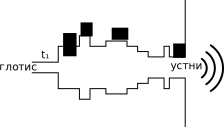
\includegraphics[width=0.7\textwidth]{vocal_tubes}%
                }
            \end{column}%
        \end{columns}
    \end{frame}

    \begin{frame}[t]{Сигнал от реч - модел на тръбите}
        \begin{columns}[T]
            \begin{column}{0.48\textwidth}
                \begin{flalign*}
                    & u_k(x, t) = \Q{u_k^+\B{t - \frac{x}{c}} - u_k^-\B{t + \frac{x}{c}}} && \\
                    & p_k(x, t) = \cfrac{\rho c}{A_k}\Q{u_k^+\B{t - \frac{x}{c}} + u_k^-\B{t + \frac{x}{c}}} &&
                \end{flalign*}
            \end{column}%
            \hfill%
            \begin{column}{0.48\textwidth}
                \centering{
                    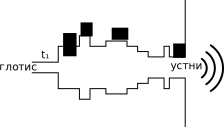
\includegraphics[width=0.7\textwidth]{vocal_tubes}%
                }
            \end{column}%
        \end{columns}
    \end{frame}

    \begin{frame}[t]{Сигнал от реч - модел на тръбите}
        \begin{columns}[T]
            \begin{column}{0.48\textwidth}
                \begin{flalign*}
                    & u_k(x, t) = \Q{u_k^+\B{t - \frac{x}{c}} - u_k^-\B{t + \frac{x}{c}}} && \\
                    & p_k(x, t) = \cfrac{\rho c}{A_k}\Q{u_k^+\B{t - \frac{x}{c}} + u_k^-\B{t + \frac{x}{c}}} &&
                \end{flalign*}
            \end{column}%
            \hfill%
            \begin{column}{0.26\textwidth}
                \begin{flalign*}
                    & u_k(l_k, t)= u_{k+1}(0, t) && \\
                    & p_k(l_k, t)= p_{k+1}(0, t) &&
                \end{flalign*}
            \end{column}%
            \hfill
            \begin{column}{0.22\textwidth}
            \end{column}%
        \end{columns}
        \pause
        \begin{flalign*}
            & u_k^+\B{t - \cfrac{l_k}{c}} - u_k^{-}\B{t + \cfrac{l_k}{c}} = u_{k+1}^{+}(t) - u_{k+1}^{-}(t) &&\\
            & \cfrac{A_{k+1}}{A_{k}}\Q{u_{k}^{+}\B{t - \cfrac{l_k}{c}} + u_{k}^{-}\B{t + \cfrac{l_k}{c}}} = u_{k+1}^{+}(t) + u_{k+1}^{-}(t) &&
        \end{flalign*}  
    \end{frame}


    \begin{frame}[t]{Сигнал от реч - модел на тръбите}
        \begin{columns}[T]
            \begin{column}{0.48\textwidth}
                \begin{flalign*}
                    & u_k(x, t) = \Q{u_k^+\B{t - \frac{x}{c}} - u_k^-\B{t + \frac{x}{c}}} && \\
                    & p_k(x, t) = \cfrac{\rho c}{A_k}\Q{u_k^+\B{t - \frac{x}{c}} + u_k^-\B{t + \frac{x}{c}}} &&
                \end{flalign*}
            \end{column}%
            \hfill%
            \begin{column}{0.26\textwidth}
                \begin{flalign*}
                    & u_k(l_k, t)= u_{k+1}(0, t) && \\
                    & p_k(l_k, t)= p_{k+1}(0, t) &&
                \end{flalign*}
            \end{column}%
            \hfill
            \begin{column}{0.22\textwidth}
            \end{column}%
        \end{columns}
        \begin{flalign*}
            & u_k^+\B{t - \cfrac{l_k}{c}} - u_k^{-}\B{t + \cfrac{l_k}{c}} = u_{k+1}^{+}(t) - u_{k+1}^{-}(t) &&\\
            & \cfrac{A_{k+1}}{A_{k}}\Q{u_{k}^{+}\B{t - \cfrac{l_k}{c}} + u_{k}^{-}\B{t + \cfrac{l_k}{c}}} = u_{k+1}^{+}(t) + u_{k+1}^{-}(t) \qquad \tau_k = \cfrac{l_k}{c} &&
        \end{flalign*}  
    \end{frame}

    \begin{frame}[t]{Сигнал от реч - модел на тръбите}
        \begin{columns}[T]
            \begin{column}{0.48\textwidth}
                \begin{flalign*}
                    & u_k(x, t) = \Q{u_k^+\B{t - \frac{x}{c}} - u_k^-\B{t + \frac{x}{c}}} && \\
                    & p_k(x, t) = \cfrac{\rho c}{A_k}\Q{u_k^+\B{t - \frac{x}{c}} + u_k^-\B{t + \frac{x}{c}}} &&
                \end{flalign*}
            \end{column}%
            \hfill%
            \begin{column}{0.26\textwidth}
                \begin{flalign*}
                    & u_k(l_k, t) = u_{k+1}(0, t) && \\
                    & p_k(l_k, t) = p_{k+1}(0, t) &&
                \end{flalign*}
            \end{column}%
            \hfill
            \begin{column}{0.22\textwidth}
            \end{column}%
        \end{columns}
        \begin{flalign*}
            & u_k^+\B{t - \tau_k} - u_k^{-}\B{t + \tau_k} = u_{k+1}^{+}(t) - u_{k+1}^{-}(t) &&\\
            & \cfrac{A_{k+1}}{A_{k}}\Q{u_{k}^{+}\B{t - \tau_k} + u_{k}^{-}\B{t + \tau_k}} = u_{k+1}^{+}(t) + u_{k+1}^{-}(t) &&
        \end{flalign*}
    \end{frame}


    \begin{frame}[t]{Сигнал от реч - модел на тръбите}
        \begin{columns}[T]
            \begin{column}{0.48\textwidth}
                \begin{flalign*}
                    & u_k(x, t) = \Q{u_k^+\B{t - \frac{x}{c}} - u_k^-\B{t + \frac{x}{c}}} && \\
                    & p_k(x, t) = \cfrac{\rho c}{A_k}\Q{u_k^+\B{t - \frac{x}{c}} + u_k^-\B{t + \frac{x}{c}}} &&
                \end{flalign*}
            \end{column}%
            \hfill%
            \begin{column}{0.26\textwidth}
                \begin{flalign*}
                    & u_k(l_k, t) = u_{k+1}(0, t) && \\
                    & p_k(l_k, t) = p_{k+1}(0, t) &&
                \end{flalign*}
            \end{column}%
            \hfill
            \begin{column}{0.22\textwidth}
            \end{column}%
        \end{columns}
        \begin{flalign*}
            & {\color{mypink}u_k^+\B{t - \tau_k} - \boldsymbol{u_k^{-}\B{t + \tau_k}} = u_{k+1}^{+}(t) - u_{k+1}^{-}(t)} &&\\
            & \cfrac{A_{k+1}}{A_{k}}\Q{u_{k}^{+}\B{t - \tau_k} + u_{k}^{-}\B{t + \tau_k}} = u_{k+1}^{+}(t) + u_{k+1}^{-}(t) &&
        \end{flalign*}
        \pause
        \begin{flalign*}
            & u_k^{-}\B{t + \tau_k} = u_k^+\B{t - \tau_k} - u_{k+1}^{+}(t) + u_{k+1}^{-}(t) &&
        \end{flalign*}
        \vspace{1.7cm}
    \end{frame}


    \begin{frame}[t]{Сигнал от реч - модел на тръбите}
        \begin{columns}[T]
            \begin{column}{0.48\textwidth}
                \begin{flalign*}
                    & u_k(x, t) = \Q{u_k^+\B{t - \frac{x}{c}} - u_k^-\B{t + \frac{x}{c}}} && \\
                    & p_k(x, t) = \cfrac{\rho c}{A_k}\Q{u_k^+\B{t - \frac{x}{c}} + u_k^-\B{t + \frac{x}{c}}} &&
                \end{flalign*}
            \end{column}%
            \hfill%
            \begin{column}{0.26\textwidth}
                \begin{flalign*}
                    & u_k(l_k, t) = u_{k+1}(0, t) && \\
                    & p_k(l_k, t) = p_{k+1}(0, t) &&
                \end{flalign*}
            \end{column}%
            \hfill
            \begin{column}{0.22\textwidth}
            \end{column}%
        \end{columns}
        \begin{flalign*}
            & u_k^+\B{t - \tau_k} - u_k^{-}\B{t + \tau_k} = u_{k+1}^{+}(t) - u_{k+1}^{-}(t) &&\\
            & {\color{mypink}\cfrac{A_{k+1}}{A_{k}}\Q{u_{k}^{+}\B{t - \tau_k} + \boldsymbol{u_{k}^{-}\B{t + \tau_k}}} = u_{k+1}^{+}(t) + u_{k+1}^{-}(t)} &&
        \end{flalign*}
        \begin{flalign*}
            & {\color{mypink} \boldsymbol{u_k^{-}\B{t + \tau_k}}} = u_k^+\B{t - \tau_k} - u_{k+1}^{+}(t) + u_{k+1}^{-}(t) &&
        \end{flalign*}
        и изразяваме $u_{k+1}^{+}$
    \end{frame}
    
    \begin{frame}[t]{Сигнал от реч - модел на тръбите}
        \begin{columns}[T]
            \begin{column}{0.48\textwidth}
                \begin{flalign*}
                    & u_k(x, t) = \Q{u_k^+\B{t - \frac{x}{c}} - u_k^-\B{t + \frac{x}{c}}} && \\
                    & p_k(x, t) = \cfrac{\rho c}{A_k}\Q{u_k^+\B{t - \frac{x}{c}} + u_k^-\B{t + \frac{x}{c}}} &&
                \end{flalign*}
            \end{column}%
            \hfill%
            \begin{column}{0.26\textwidth}
                \begin{flalign*}
                    & u_k(l_k, t) = u_{k+1}(0, t) && \\
                    & p_k(l_k, t) = p_{k+1}(0, t) &&
                \end{flalign*}
            \end{column}%
            \hfill
            \begin{column}{0.22\textwidth}
            \end{column}%
        \end{columns}
        \begin{flalign*}
            & u_k^+\B{t - \tau_k} - u_k^{-}\B{t + \tau_k} = u_{k+1}^{+}(t) - u_{k+1}^{-}(t) &&\\
            & \cfrac{A_{k+1}}{A_{k}}\Q{u_{k}^{+}\B{t - \tau_k} + u_{k}^{-}\B{t + \tau_k} = u_{k+1}^{+}(t) + u_{k+1}^{-}(t)} &&
        \end{flalign*}
        \begin{flalign*}
            & u_k^{-}\B{t + \tau_k} = u_k^+\B{t - \tau_k} - u_{k+1}^{+}(t) + u_{k+1}^{-}(t) &&\\
            & u_{k+1}^{+}(t) = u_{k}^{+}(t - \tau_k)\Q{\frac{2A_{k+1}}{A_k + A_{k+1}}} + u_{k+1}^{-}(t)\Q{\frac{A_{k+1} - A_k}{A_k + A_{k+1}}} &&
        \end{flalign*}
        \pause
        \begin{columns}[T]
            \begin{column}{0.48\textwidth}
                $t_k = \cfrac{2A_{k+1}}{A_k + A_{k+1}}$
            \end{column}%
            \hfill%
            \pause
            \begin{column}{0.48\textwidth}
                $r_k = \cfrac{A_{k+1} - A_k}{A_k + A_{k+1}}$
            \end{column}%
        \end{columns}
    \end{frame}

    \begin{frame}[t]{Сигнал от реч - модел на тръбите}
        \begin{columns}[T]
            \begin{column}{0.48\textwidth}
                \begin{flalign*}
                    & u_k(x, t) = \Q{u_k^+\B{t - \frac{x}{c}} - u_k^-\B{t + \frac{x}{c}}} && \\
                    & p_k(x, t) = \cfrac{\rho c}{A_k}\Q{u_k^+\B{t - \frac{x}{c}} + u_k^-\B{t + \frac{x}{c}}} &&
                \end{flalign*}
            \end{column}%
            \hfill%
            \begin{column}{0.26\textwidth}
                \begin{flalign*}
                    & u_k(l_k, t) = u_{k+1}(0, t) && \\
                    & p_k(l_k, t) = p_{k+1}(0, t) &&
                \end{flalign*}
            \end{column}%
            \hfill
            \begin{column}{0.22\textwidth}
                \begin{flalign*}
                    & r_k = \cfrac{A_{k+1} - A_k}{A_k + A_{k+1}} &&
                \end{flalign*}
            \end{column}%
        \end{columns}
        \begin{flalign*}
            & u_k^+\B{t - \tau_k} - u_k^{-}\B{t + \tau_k} = u_{k+1}^{+}(t) - u_{k+1}^{-}(t) &&\\
            & \cfrac{A_{k+1}}{A_{k}}\Q{u_{k}^{+}\B{t - \tau_k} + u_{k}^{-}\B{t + \tau_k} = u_{k+1}^{+}(t) + u_{k+1}^{-}(t)} &&
        \end{flalign*}
        \begin{flalign*}
            & u_k^{-}\B{t + \tau_k} = u_k^+\B{t - \tau_k} - u_{k+1}^{+}(t) + u_{k+1}^{-}(t) &&\\
            & u_{k+1}^{+}(t) = u_{k}^{+}(t - \tau_k)\Q{\frac{2A_{k+1}}{A_k + A_{k+1}}} + u_{k+1}^{-}(t)\Q{\frac{A_{k+1} - A_k}{A_k + A_{k+1}}} &&
        \end{flalign*}
        \begin{columns}[T]
            \begin{column}{0.48\textwidth}
                $t_k = \cfrac{2A_{k+1}}{A_k + A_{k+1}}$
            \end{column}%
            \hfill%
            \begin{column}{0.48\textwidth}
                $r_k = \cfrac{A_{k+1} - A_k}{A_k + A_{k+1}}$
            \end{column}%
        \end{columns}
    \end{frame}

        
    \begin{frame}[t]{Сигнал от реч - модел на тръбите}
        \begin{columns}[T]
            \begin{column}{0.48\textwidth}
                \begin{flalign*}
                    & u_k(x, t) = \Q{u_k^+\B{t - \frac{x}{c}} - u_k^-\B{t + \frac{x}{c}}} && \\
                    & p_k(x, t) = \cfrac{\rho c}{A_k}\Q{u_k^+\B{t - \frac{x}{c}} + u_k^-\B{t + \frac{x}{c}}} &&
                \end{flalign*}
            \end{column}%
            \hfill%
            \begin{column}{0.26\textwidth}
                \begin{flalign*}
                    & u_k(l_k, t) = u_{k+1}(0, t) && \\
                    & p_k(l_k, t) = p_{k+1}(0, t) &&
                \end{flalign*}
            \end{column}%
            \hfill
            \begin{column}{0.22\textwidth}
                \begin{flalign*}
                    & r_k = \cfrac{A_{k+1} - A_k}{A_k + A_{k+1}} &&
                \end{flalign*}
            \end{column}%
        \end{columns}
        \begin{flalign*}
            & u_k^+\B{t - \tau_k} - u_k^{-}\B{t + \tau_k} = u_{k+1}^{+}(t) - u_{k+1}^{-}(t) &&\\
            & \cfrac{A_{k+1}}{A_{k}}\Q{u_{k}^{+}\B{t - \tau_k} + u_{k}^{-}\B{t + \tau_k} = u_{k+1}^{+}(t) + u_{k+1}^{-}(t)} &&
        \end{flalign*}
        \begin{flalign*}
            & u_k^{-}\B{t + \tau_k} = u_k^+\B{t - \tau_k} - u_{k+1}^{+}(t) + u_{k+1}^{-}(t) &&\\
            & {\color{mypink}u_{k+1}^{+}(t) = u_{k}^{+}(t - \tau_k)\Q{\frac{2A_{k+1}}{A_k + A_{k+1}}} + u_{k+1}^{-}(t)\Q{\frac{A_{k+1} - A_k}{A_k + A_{k+1}}}} &&
        \end{flalign*}
    \end{frame}
            
    \begin{frame}[t]{Сигнал от реч - модел на тръбите}
        \begin{columns}[T]
            \begin{column}{0.48\textwidth}
                \begin{flalign*}
                    & u_k(x, t) = \Q{u_k^+\B{t - \frac{x}{c}} - u_k^-\B{t + \frac{x}{c}}} && \\
                    & p_k(x, t) = \cfrac{\rho c}{A_k}\Q{u_k^+\B{t - \frac{x}{c}} + u_k^-\B{t + \frac{x}{c}}} &&
                \end{flalign*}
            \end{column}%
            \hfill%
            \begin{column}{0.26\textwidth}
                \begin{flalign*}
                    & u_k(l_k, t) = u_{k+1}(0, t) && \\
                    & p_k(l_k, t) = p_{k+1}(0, t) &&
                \end{flalign*}
            \end{column}%
            \hfill
            \begin{column}{0.22\textwidth}
                \begin{flalign*}
                    & r_k = \cfrac{A_{k+1} - A_k}{A_k + A_{k+1}} &&
                \end{flalign*}
            \end{column}%
        \end{columns}
        \begin{flalign*}
            & u_k^+\B{t - \tau_k} - u_k^{-}\B{t + \tau_k} = u_{k+1}^{+}(t) - u_{k+1}^{-}(t) &&\\
            & \cfrac{A_{k+1}}{A_{k}}\Q{u_{k}^{+}\B{t - \tau_k} + u_{k}^{-}\B{t + \tau_k} = u_{k+1}^{+}(t) + u_{k+1}^{-}(t)} &&
        \end{flalign*}
        \begin{flalign*}
            & {\color{mypink}u_{k+1}^{+}(t) = \boldsymbol{u_{k}^{+}(t - \tau_k)}\Q{\frac{2A_{k+1}}{A_k + A_{k+1}}} + u_{k+1}^{-}(t)\Q{\frac{A_{k+1} - A_k}{A_k + A_{k+1}}}} &&
        \end{flalign*}
    \end{frame}
    
    \begin{frame}[t]{Сигнал от реч - модел на тръбите}
        \begin{columns}[T]
            \begin{column}{0.48\textwidth}
                \begin{flalign*}
                    & u_k(x, t) = \Q{u_k^+\B{t - \frac{x}{c}} - u_k^-\B{t + \frac{x}{c}}} && \\
                    & p_k(x, t) = \cfrac{\rho c}{A_k}\Q{u_k^+\B{t - \frac{x}{c}} + u_k^-\B{t + \frac{x}{c}}} &&
                \end{flalign*}
            \end{column}%
            \hfill%
            \begin{column}{0.26\textwidth}
                \begin{flalign*}
                    & u_k(l_k, t) = u_{k+1}(0, t) && \\
                    & p_k(l_k, t) = p_{k+1}(0, t) &&
                \end{flalign*}
            \end{column}%
            \hfill
            \begin{column}{0.22\textwidth}
                \begin{flalign*}
                    & r_k = \cfrac{A_{k+1} - A_k}{A_k + A_{k+1}} &&
                \end{flalign*}
            \end{column}%
        \end{columns}
        \begin{flalign*}
            & u_k^+\B{t - \tau_k} - u_k^{-}\B{t + \tau_k} = u_{k+1}^{+}(t) - u_{k+1}^{-}(t) &&\\
            & \cfrac{A_{k+1}}{A_{k}}\Q{u_{k}^{+}\B{t - \tau_k} + u_{k}^{-}\B{t + \tau_k} = u_{k+1}^{+}(t) + u_{k+1}^{-}(t)} &&
        \end{flalign*}
        \begin{flalign*}
            & {\color{mypink}u_{k+1}^{+}(t) = \boldsymbol{u_{k}^{+}(t - \tau_k)}\Q{\frac{2A_{k+1}}{A_k + A_{k+1}}} + u_{k+1}^{-}(t)\Q{\frac{A_{k+1} - A_k}{A_k + A_{k+1}}}} && \\
            & u_k^{+}(t - \tau_k) = u_{k+1}^{+}(t)\Q{\frac{A_k + A_{k+1}}{2A_{k+1}}} + u_{k+1}^{-}(t)\Q{\frac{A_k - A_{k+1}}{2A_{k+1}}} &&
        \end{flalign*}
    \end{frame}

    \begin{frame}[t]{Сигнал от реч - модел на тръбите}
    \begin{columns}[T]
        \begin{column}{0.48\textwidth}
            \begin{flalign*}
                & u_k(x, t) = \Q{u_k^+\B{t - \frac{x}{c}} - u_k^-\B{t + \frac{x}{c}}} && \\
                & p_k(x, t) = \cfrac{\rho c}{A_k}\Q{u_k^+\B{t - \frac{x}{c}} + u_k^-\B{t + \frac{x}{c}}} &&
            \end{flalign*}
        \end{column}%
        \hfill%
        \begin{column}{0.26\textwidth}
            \begin{flalign*}
                & u_k(l_k, t) = u_{k+1}(0, t) && \\
                & p_k(l_k, t) = p_{k+1}(0, t) &&
            \end{flalign*}
        \end{column}%
        \hfill
        \begin{column}{0.22\textwidth}
            \begin{flalign*}
                & r_k = \cfrac{A_{k+1} - A_k}{A_k + A_{k+1}} &&
            \end{flalign*}
        \end{column}%
    \end{columns}
    \begin{flalign*}
        & u_k^+\B{t - \tau_k} - u_k^{-}\B{t + \tau_k} = u_{k+1}^{+}(t) - u_{k+1}^{-}(t) &&\\
        & \cfrac{A_{k+1}}{A_{k}}\Q{u_{k}^{+}\B{t - \tau_k} + u_{k}^{-}\B{t + \tau_k} = u_{k+1}^{+}(t) + u_{k+1}^{-}(t)} &&
    \end{flalign*}
    \begin{flalign*}
        & u_{k+1}^{+}(t) = u_{k}^{+}(t - \tau_k)\Q{\frac{2A_{k+1}}{A_k + A_{k+1}}} + u_{k+1}^{-}(t)\Q{\frac{A_{k+1} - A_k}{A_k + A_{k+1}}} && \\
        & u_k^{+}(t - \tau_k) = u_{k+1}^{+}(t)\Q{\frac{A_k + A_{k+1}}{2A_{k+1}}} + u_{k+1}^{-}(t)\Q{\frac{A_k - A_{k+1}}{2A_{k+1}}} &&
    \end{flalign*}
\end{frame}

\begin{frame}[t]{Сигнал от реч - модел на тръбите}
    \begin{columns}[T]
        \begin{column}{0.48\textwidth}
            \begin{flalign*}
                & u_k(x, t) = \Q{u_k^+\B{t - \frac{x}{c}} - u_k^-\B{t + \frac{x}{c}}} && \\
                & p_k(x, t) = \cfrac{\rho c}{A_k}\Q{u_k^+\B{t - \frac{x}{c}} + u_k^-\B{t + \frac{x}{c}}} &&
            \end{flalign*}
        \end{column}%
        \hfill%
        \begin{column}{0.26\textwidth}
            \begin{flalign*}
                & u_k(l_k, t) = u_{k+1}(0, t) && \\
                & p_k(l_k, t) = p_{k+1}(0, t) &&
            \end{flalign*}
        \end{column}%
        \hfill
        \begin{column}{0.22\textwidth}
            \begin{flalign*}
                & r_k = \cfrac{A_{k+1} - A_k}{A_k + A_{k+1}} &&
            \end{flalign*}
        \end{column}%
    \end{columns}
    \begin{flalign*}
        & {\color{mypink} u_k^+\B{t - \tau_k} - \boldsymbol{u_k^{-}\B{t + \tau_k}} = u_{k+1}^{+}(t) - u_{k+1}^{-}(t)} &&\\
        & \cfrac{A_{k+1}}{A_{k}}\Q{u_{k}^{+}\B{t - \tau_k} + u_{k}^{-}\B{t + \tau_k} = u_{k+1}^{+}(t) + u_{k+1}^{-}(t)} &&
    \end{flalign*}
    \begin{flalign*}
        & u_{k+1}^{+}(t) = u_{k}^{+}(t - \tau_k)\Q{\frac{2A_{k+1}}{A_k + A_{k+1}}} + u_{k+1}^{-}(t)\Q{\frac{A_{k+1} - A_k}{A_k + A_{k+1}}} && \\
        & {\color{mypink} u_k^{+}(t - \tau_k)} = u_{k+1}^{+}(t)\Q{\frac{A_k + A_{k+1}}{2A_{k+1}}} + u_{k+1}^{-}(t)\Q{\frac{A_k - A_{k+1}}{2A_{k+1}}} &&
    \end{flalign*}
\end{frame}

\begin{frame}[t]{Сигнал от реч - модел на тръбите}
    \begin{columns}[T]
        \begin{column}{0.48\textwidth}
            \begin{flalign*}
                & u_k(x, t) = \Q{u_k^+\B{t - \frac{x}{c}} - u_k^-\B{t + \frac{x}{c}}} && \\
                & p_k(x, t) = \cfrac{\rho c}{A_k}\Q{u_k^+\B{t - \frac{x}{c}} + u_k^-\B{t + \frac{x}{c}}} &&
            \end{flalign*}
        \end{column}%
        \hfill%
        \begin{column}{0.26\textwidth}
            \begin{flalign*}
                & u_k(l_k, t) = u_{k+1}(0, t) && \\
                & p_k(l_k, t) = p_{k+1}(0, t) &&
            \end{flalign*}
        \end{column}%
        \hfill
        \begin{column}{0.22\textwidth}
            \begin{flalign*}
                & r_k = \cfrac{A_{k+1} - A_k}{A_k + A_{k+1}} &&
            \end{flalign*}
        \end{column}%
    \end{columns}
    \begin{flalign*}
        & {\color{mypink} u_k^+\B{t - \tau_k} - \boldsymbol{u_k^{-}\B{t + \tau_k}} = u_{k+1}^{+}(t) - u_{k+1}^{-}(t)} &&\\
        & \cfrac{A_{k+1}}{A_{k}}\Q{u_{k}^{+}\B{t - \tau_k} + u_{k}^{-}\B{t + \tau_k} = u_{k+1}^{+}(t) + u_{k+1}^{-}(t)} &&
    \end{flalign*}
    \begin{flalign*}
        & u_{k+1}^{+}(t) = u_{k}^{+}(t - \tau_k)\Q{\frac{2A_{k+1}}{A_k + A_{k+1}}} + u_{k+1}^{-}(t)\Q{\frac{A_{k+1} - A_k}{A_k + A_{k+1}}} && \\
        & u_k^{+}(t - \tau_k) = u_{k+1}^{+}(t)\Q{\frac{A_k + A_{k+1}}{2A_{k+1}}} + u_{k+1}^{-}(t)\Q{\frac{A_k - A_{k+1}}{2A_{k+1}}} &&\\
        & u_k^{-}(t + \tau_k) = u_{k+1}^{+}(t)\Q{\frac{A_k - A_{k+1}}{2A_{k+1}}} + u_{k+1}^{-}(t)\Q{\frac{A_k + A_{k+1}}{2A_{k+1}}} &&
    \end{flalign*}
\end{frame}

\begin{frame}[t]{Сигнал от реч - модел на тръбите}
    \begin{columns}[T]
        \begin{column}{0.48\textwidth}
            \begin{flalign*}
                & u_k(x, t) = \Q{u_k^+\B{t - \frac{x}{c}} - u_k^-\B{t + \frac{x}{c}}} && \\
                & p_k(x, t) = \cfrac{\rho c}{A_k}\Q{u_k^+\B{t - \frac{x}{c}} + u_k^-\B{t + \frac{x}{c}}} &&
            \end{flalign*}
        \end{column}%
        \hfill%
        \begin{column}{0.26\textwidth}
            \begin{flalign*}
                & u_k(l_k, t) = u_{k+1}(0, t) && \\
                & p_k(l_k, t) = p_{k+1}(0, t) &&
            \end{flalign*}
        \end{column}%
        \hfill
        \begin{column}{0.22\textwidth}
            \begin{flalign*}
                & r_k = \cfrac{A_{k+1} - A_k}{A_k + A_{k+1}} &&
            \end{flalign*}
        \end{column}%
    \end{columns}
    \begin{flalign*}
        & u_k^+\B{t - \tau_k} - u_k^{-}\B{t + \tau_k} = u_{k+1}^{+}(t) - u_{k+1}^{-}(t) &&\\
        & \cfrac{A_{k+1}}{A_{k}}\Q{u_{k}^{+}\B{t - \tau_k} + u_{k}^{-}\B{t + \tau_k} = u_{k+1}^{+}(t) + u_{k+1}^{-}(t)} &&
    \end{flalign*}
    \begin{flalign*}
        & u_{k+1}^{+}(t) = u_{k}^{+}(t - \tau_k)\Q{\frac{2A_{k+1}}{A_k + A_{k+1}}} + u_{k+1}^{-}(t)\Q{\frac{A_{k+1} - A_k}{A_k + A_{k+1}}} && \\
        & u_k^{+}(t - \tau_k) = u_{k+1}^{+}(t)\Q{\frac{A_k + A_{k+1}}{2A_{k+1}}} + u_{k+1}^{-}(t)\Q{\frac{A_k - A_{k+1}}{2A_{k+1}}} &&\\
        & u_k^{-}(t + \tau_k) = u_{k+1}^{+}(t)\Q{\frac{A_k - A_{k+1}}{2A_{k+1}}} + u_{k+1}^{-}(t)\Q{\frac{A_k + A_{k+1}}{2A_{k+1}}} &&
    \end{flalign*}
\end{frame}

\begin{frame}[t]{Сигнал от реч - модел на тръбите}
    \begin{columns}[T]
        \begin{column}{0.48\textwidth}
            \begin{flalign*}
                & u_k(x, t) = \Q{u_k^+\B{t - \frac{x}{c}} - u_k^-\B{t + \frac{x}{c}}} && \\
                & p_k(x, t) = \cfrac{\rho c}{A_k}\Q{u_k^+\B{t - \frac{x}{c}} + u_k^-\B{t + \frac{x}{c}}} &&
            \end{flalign*}
        \end{column}%
        \hfill%
        \begin{column}{0.26\textwidth}
            \begin{flalign*}
                & u_k(l_k, t) = u_{k+1}(0, t) && \\
                & p_k(l_k, t) = p_{k+1}(0, t) &&
            \end{flalign*}
        \end{column}%
        \hfill
        \begin{column}{0.22\textwidth}
            \begin{flalign*}
                & r_k = \cfrac{A_{k+1} - A_k}{A_k + A_{k+1}} &&
            \end{flalign*}
        \end{column}%
    \end{columns}
    \begin{flalign*}
        & u_k^+\B{t - \tau_k} - u_k^{-}\B{t + \tau_k} = u_{k+1}^{+}(t) - u_{k+1}^{-}(t) &&\\
        & \cfrac{A_{k+1}}{A_{k}}\Q{u_{k}^{+}\B{t - \tau_k} + u_{k}^{-}\B{t + \tau_k} = u_{k+1}^{+}(t) + u_{k+1}^{-}(t)} &&
    \end{flalign*}
    \begin{flalign*}
        & u_{k+1}^{+}(t) = u_{k}^{+}(t - \tau_k)\Q{\frac{2A_{k+1}}{A_k + A_{k+1}}} + u_{k+1}^{-}(t)\Q{\frac{A_{k+1} - A_k}{A_k + A_{k+1}}} && \\
        & {\color{mypink} u_k^{+}(t - \tau_k) = u_{k+1}^{+}(t)\Q{\frac{A_k + A_{k+1}}{2A_{k+1}}} + u_{k+1}^{-}(t)\Q{\frac{A_k - A_{k+1}}{2A_{k+1}}}} &&\\
        & {\color{mypink} u_k^{-}(t + \tau_k) = u_{k+1}^{+}(t)\Q{\frac{A_k - A_{k+1}}{2A_{k+1}}} + u_{k+1}^{-}(t)\Q{\frac{A_k + A_{k+1}}{2A_{k+1}}}} &&
    \end{flalign*}
\end{frame}

\begin{frame}[t]{Сигнал от реч - модел на тръбите}
    \begin{columns}[T]
        \begin{column}{0.48\textwidth}
            \begin{flalign*}
                & u_k(x, t) = \Q{u_k^+\B{t - \frac{x}{c}} - u_k^-\B{t + \frac{x}{c}}} && \\
                & p_k(x, t) = \cfrac{\rho c}{A_k}\Q{u_k^+\B{t - \frac{x}{c}} + u_k^-\B{t + \frac{x}{c}}} &&
            \end{flalign*}
        \end{column}%
        \hfill%
        \begin{column}{0.26\textwidth}
            \begin{flalign*}
                & u_k(l_k, t) = u_{k+1}(0, t) && \\
                & p_k(l_k, t) = p_{k+1}(0, t) &&
            \end{flalign*}
        \end{column}%
        \hfill
        \begin{column}{0.22\textwidth}
            \begin{flalign*}
                & r_k = \cfrac{A_{k+1} - A_k}{A_k + A_{k+1}} &&
            \end{flalign*}
        \end{column}%
    \end{columns}
    \begin{flalign*}
        & u_k^{+}(t - \tau_k) = u_{k+1}^{+}(t)\Q{\frac{A_k + A_{k+1}}{2A_{k+1}}} + u_{k+1}^{-}(t)\Q{\frac{A_k - A_{k+1}}{2A_{k+1}}} &&\\
        & u_k^{-}(t + \tau_k) = u_{k+1}^{+}(t)\Q{\frac{A_k - A_{k+1}}{2A_{k+1}}} + u_{k+1}^{-}(t)\Q{\frac{A_k + A_{k+1}}{2A_{k+1}}} &&
    \end{flalign*}
\end{frame}

\begin{frame}[t]{Сигнал от реч - модел на тръбите}
    \begin{columns}[T]
        \begin{column}{0.48\textwidth}
            \begin{flalign*}
                & u_k(x, t) = \Q{u_k^+\B{t - \frac{x}{c}} - u_k^-\B{t + \frac{x}{c}}} && \\
                & p_k(x, t) = \cfrac{\rho c}{A_k}\Q{u_k^+\B{t - \frac{x}{c}} + u_k^-\B{t + \frac{x}{c}}} &&
            \end{flalign*}
        \end{column}%
        \hfill%
        \begin{column}{0.26\textwidth}
            \begin{flalign*}
                & u_k(l_k, t) = u_{k+1}(0, t) && \\
                & p_k(l_k, t) = p_{k+1}(0, t) &&
            \end{flalign*}
        \end{column}%
        \hfill
        \begin{column}{0.22\textwidth}
            \begin{flalign*}
                & {\color{mypink}r_k = \cfrac{A_{k+1} - A_k}{A_k + A_{k+1}}} &&
            \end{flalign*}
        \end{column}%
    \end{columns}
    \begin{flalign*}
        & u_k^{+}(t - \tau_k) = u_{k+1}^{+}(t)\Q{\frac{A_k + A_{k+1}}{2A_{k+1}}} + u_{k+1}^{-}(t)\Q{\frac{A_k - A_{k+1}}{2A_{k+1}}} &&\\
        & u_k^{-}(t + \tau_k) = u_{k+1}^{+}(t)\Q{\frac{A_k - A_{k+1}}{2A_{k+1}}} + u_{k+1}^{-}(t)\Q{\frac{A_k + A_{k+1}}{2A_{k+1}}} &&
    \end{flalign*}
\end{frame}

\begin{frame}[t]{Сигнал от реч - модел на тръбите}
    \begin{columns}[T]
        \begin{column}{0.48\textwidth}
            \begin{flalign*}
                & u_k(x, t) = \Q{u_k^+\B{t - \frac{x}{c}} - u_k^-\B{t + \frac{x}{c}}} && \\
                & p_k(x, t) = \cfrac{\rho c}{A_k}\Q{u_k^+\B{t - \frac{x}{c}} + u_k^-\B{t + \frac{x}{c}}} &&
            \end{flalign*}
        \end{column}%
        \hfill%
        \begin{column}{0.26\textwidth}
            \begin{flalign*}
                & u_k(l_k, t) = u_{k+1}(0, t) && \\
                & p_k(l_k, t) = p_{k+1}(0, t) &&
            \end{flalign*}
        \end{column}%
        \hfill
        \begin{column}{0.22\textwidth}
            \begin{flalign*}
                & {\color{mypink}r_k = \cfrac{A_{k+1} - A_k}{A_k + A_{k+1}}} &&
            \end{flalign*}
        \end{column}%
    \end{columns}
    \begin{flalign*}
        & u_k^{+}(t - \tau_k) = \cfrac{1}{1 + r_k} u_{k+1}^{+}(t) - \cfrac{r_k}{1+r_k} u_{k+1}^{-}(t) && \\
        & u_k^{-}(t + \tau_k) = - \cfrac{r_k}{1+r_k} u_{k+1}^{+}(t) + \cfrac{1}{1 + r_k} u_{k+1}^{-}(t) &&
    \end{flalign*}
\end{frame}

\begin{frame}[t]{Сигнал от реч - модел на тръбите}
    \begin{columns}[T]
        \begin{column}{0.48\textwidth}
            \begin{flalign*}
                & u_k(x, t) = \Q{u_k^+\B{t - \frac{x}{c}} - u_k^-\B{t + \frac{x}{c}}} && \\
                & p_k(x, t) = \cfrac{\rho c}{A_k}\Q{u_k^+\B{t - \frac{x}{c}} + u_k^-\B{t + \frac{x}{c}}} &&
            \end{flalign*}
        \end{column}%
        \hfill%
        \begin{column}{0.26\textwidth}
            \begin{flalign*}
                & u_k(l_k, t) = u_{k+1}(0, t) && \\
                & p_k(l_k, t) = p_{k+1}(0, t) &&
            \end{flalign*}
        \end{column}%
        \hfill
        \begin{column}{0.22\textwidth}
            \begin{flalign*}
                & r_k = \cfrac{A_{k+1} - A_k}{A_k + A_{k+1}} &&
            \end{flalign*}
        \end{column}%
    \end{columns}
    \begin{flalign*}
        & u_k^{+}(t - \tau_k) = \cfrac{1}{1 + r_k} u_{k+1}^{+}(t) - \cfrac{r_k}{1+r_k} u_{k+1}^{-}(t) && \\
        & u_k^{-}(t + \tau_k) = - \cfrac{r_k}{1+r_k} u_{k+1}^{+}(t) + \cfrac{1}{1 + r_k} u_{k+1}^{-}(t) &&
    \end{flalign*}
    \pause
    Нека $u_k(t) \xleftrightarrow{\mathcal{F}\mathcal{S}} U_k(z)$.
    \pause
        
    Тогава $u_k(t - \tau_k) \xleftrightarrow{\mathcal{F}\mathcal{S}} z^{-\tau_k}U_k(z)$.
    \pause

    \begin{flalign*}
        & U_k^{+}(z) = \cfrac{ z^{\tau_k}}{1 + r_k} U_{k+1}^{+}( z) - \cfrac{r_k z^{\tau_k}}{1+r_k} U_{k+1}^{-}(z) && \\
        & U_k^{-}(z) = - \cfrac{r_k z^{-\tau_k} }{1+r_k} U_{k+1}^{+}( z) + \cfrac{ z^{-\tau_k} }{1 + r_k} U_{k+1}^{-}(z) &&
    \end{flalign*}
\end{frame}

\begin{frame}[t]{Сигнал от реч - модел на тръбите}
    \begin{columns}[T]
        \begin{column}{0.48\textwidth}
            \begin{flalign*}
                & u_k(x, t) = \Q{u_k^+\B{t - \frac{x}{c}} - u_k^-\B{t + \frac{x}{c}}} && \\
                & p_k(x, t) = \cfrac{\rho c}{A_k}\Q{u_k^+\B{t - \frac{x}{c}} + u_k^-\B{t + \frac{x}{c}}} &&
            \end{flalign*}
        \end{column}%
        \hfill%
        \begin{column}{0.26\textwidth}
            \begin{flalign*}
                & u_k(l_k, t) = u_{k+1}(0, t) && \\
                & p_k(l_k, t) = p_{k+1}(0, t) &&
            \end{flalign*}
        \end{column}%
        \hfill
        \begin{column}{0.22\textwidth}
            \begin{flalign*}
                & r_k = \cfrac{A_{k+1} - A_k}{A_k + A_{k+1}} &&
            \end{flalign*}
        \end{column}%
    \end{columns}
    \begin{flalign*}
        & u_k^{+}(t - \tau_k) = \cfrac{1}{1 + r_k} u_{k+1}^{+}(t) - \cfrac{r_k}{1+r_k} u_{k+1}^{-}(t) && \\
        & u_k^{-}(t + \tau_k) = - \cfrac{r_k}{1+r_k} u_{k+1}^{+}(t) + \cfrac{1}{1 + r_k} u_{k+1}^{-}(t) &&
    \end{flalign*}
    Нека $u_k(t) \xleftrightarrow{\mathcal{F}\mathcal{S}} U_k(z)$.
        
    Тогава $u_k(t - \tau_k) \xleftrightarrow{\mathcal{F}\mathcal{S}} z^{-\tau_k}U_k(z)$.

    \begin{flalign*}
        & U_k^{+}(z) = \cfrac{ z^{\tau_k}}{1 + r_k} U_{k+1}^{+}( z) - \cfrac{r_k z^{\tau_k}}{1+r_k} U_{k+1}^{-}(z) && \\
        & U_k^{-}(z) = - \cfrac{r_k z^{-\tau_k} }{1+r_k} U_{k+1}^{+}( z) + \cfrac{ z^{-\tau_k} }{1 + r_k} U_{k+1}^{-}(z) \qquad \tau_k = 1/2&&
    \end{flalign*}
\end{frame}

\begin{frame}[t]{Сигнал от реч - модел на тръбите}
    \begin{columns}[T]
        \begin{column}{0.48\textwidth}
            \begin{flalign*}
                & u_k(x, t) = \Q{u_k^+\B{t - \frac{x}{c}} - u_k^-\B{t + \frac{x}{c}}} && \\
                & p_k(x, t) = \cfrac{\rho c}{A_k}\Q{u_k^+\B{t - \frac{x}{c}} + u_k^-\B{t + \frac{x}{c}}} &&
            \end{flalign*}
        \end{column}%
        \hfill%
        \begin{column}{0.26\textwidth}
            \begin{flalign*}
                & u_k(l_k, t) = u_{k+1}(0, t) && \\
                & p_k(l_k, t) = p_{k+1}(0, t) &&
            \end{flalign*}
        \end{column}%
        \hfill
        \begin{column}{0.22\textwidth}
            \begin{flalign*}
                & r_k = \cfrac{A_{k+1} - A_k}{A_k + A_{k+1}} &&
            \end{flalign*}
        \end{column}%
    \end{columns}
    \begin{flalign*}
        & u_k^{+}(t - \tau_k) = \cfrac{1}{1 + r_k} u_{k+1}^{+}(t) - \cfrac{r_k}{1+r_k} u_{k+1}^{-}(t) && \\
        & u_k^{-}(t + \tau_k) = - \cfrac{r_k}{1+r_k} u_{k+1}^{+}(t) + \cfrac{1}{1 + r_k} u_{k+1}^{-}(t) &&
    \end{flalign*}
    Нека $u_k(t) \xleftrightarrow{\mathcal{F}\mathcal{S}} U_k(z)$.
        
    Тогава $u_k(t - \tau_k) \xleftrightarrow{\mathcal{F}\mathcal{S}} z^{-\tau_k}U_k(z)$.

    \begin{flalign*}
        & U_k^{+}(z) = \cfrac{ z^{1/2}}{1 + r_k} U_{k+1}^{+}(z) - \cfrac{r_k z^{1/2}}{1+r_k} U_{k+1}^{-}(z) && \\
        & U_k^{-}(z) = - \cfrac{r_k z^{-1/2} }{1+r_k} U_{k+1}^{+}(z) + \cfrac{ z^{-1/2} }{1 + r_k} U_{k+1}^{-}(z)&&
    \end{flalign*}
\end{frame}

\begin{frame}[t]{Сигнал от реч - модел на тръбите}
    \begin{columns}[T]
        \begin{column}{0.48\textwidth}
            \begin{flalign*}
                & u_k(x, t) = \Q{u_k^+\B{t - \frac{x}{c}} - u_k^-\B{t + \frac{x}{c}}} && \\
                & p_k(x, t) = \cfrac{\rho c}{A_k}\Q{u_k^+\B{t - \frac{x}{c}} + u_k^-\B{t + \frac{x}{c}}} &&\\
                & U_k^{+}(z) = \cfrac{ z^{1/2}}{1 + r_k} U_{k+1}^{+}(z) - \cfrac{r_k z^{1/2}}{1+r_k} U_{k+1}^{-}(z) && \\
                & U_k^{-}(z) = - \cfrac{r_k z^{-1/2} }{1+r_k} U_{k+1}^{+}(z) + \cfrac{ z^{-1/2} }{1 + r_k} U_{k+1}^{-}(z)&&
            \end{flalign*}
        \end{column}%
        \hfill%
        \begin{column}{0.24\textwidth}
        \end{column}%
        \hfill%
        \begin{column}{0.24\textwidth}
        \end{column}%
    \end{columns}
    \centering{Огрнаничения при устните}
\end{frame}

\begin{frame}[t]{Сигнал от реч - модел на тръбите}
    \begin{columns}[T]
        \begin{column}{0.48\textwidth}
            {\tiny \begin{flalign*}
                & u_k(x, t) = \Q{u_k^+\B{t - \frac{x}{c}} - u_k^-\B{t + \frac{x}{c}}} && \\
                & p_k(x, t) = \cfrac{\rho c}{A_k}\Q{u_k^+\B{t - \frac{x}{c}} + u_k^-\B{t + \frac{x}{c}}} &&\\
                & U_k^{+}(z) = \cfrac{ z^{1/2}}{1 + r_k} U_{k+1}^{+}(z) - \cfrac{r_k z^{1/2}}{1+r_k} U_{k+1}^{-}(z) && \\
                & U_k^{-}(z) = - \cfrac{r_k z^{-1/2} }{1+r_k} U_{k+1}^{+}(z) + \cfrac{ z^{-1/2} }{1 + r_k} U_{k+1}^{-}(z)&&
            \end{flalign*}}
        \end{column}%
        \hfill%
        \begin{column}{0.24\textwidth}
        \end{column}%
        \hfill%
        \begin{column}{0.24\textwidth}
        \end{column}%
    \end{columns}
    \centering{Огрнаничения при устните}
\end{frame}

\begin{frame}[t]{Сигнал от реч - модел на тръбите}
    \begin{columns}[T]
        \begin{column}{0.48\textwidth}
            {\tiny \begin{flalign*}
                & u_k(x, t) = \Q{u_k^+\B{t - \frac{x}{c}} - u_k^-\B{t + \frac{x}{c}}} && \\
                & p_k(x, t) = \cfrac{\rho c}{A_k}\Q{u_k^+\B{t - \frac{x}{c}} + u_k^-\B{t + \frac{x}{c}}} &&\\
                & U_k^{+}(z) = \cfrac{ z^{1/2}}{1 + r_k} U_{k+1}^{+}(z) - \cfrac{r_k z^{1/2}}{1+r_k} U_{k+1}^{-}(z) && \\
                & U_k^{-}(z) = - \cfrac{r_k z^{-1/2} }{1+r_k} U_{k+1}^{+}(z) + \cfrac{ z^{-1/2} }{1 + r_k} U_{k+1}^{-}(z)&&
            \end{flalign*}}
        \end{column}%
        \hfill%
        \begin{column}{0.24\textwidth}
        \end{column}%
        \hfill%
        \begin{column}{0.24\textwidth}
        \end{column}%
    \end{columns}
    \centering{Огрнаничения при устните}
    \begin{columns}[T]
        \begin{column}{0.48\textwidth}
            
\includegraphics[width=0.55\textwidth]{lips_a}%
        \end{column}
        \hfill
        \pause
        \begin{column}{0.48\textwidth}
            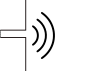
\includegraphics[width=0.55\textwidth]{lips_b}%
        \end{column}
    \end{columns}
        \pause
        \begin{flalign*}
            & \mathcal{P}_N(l_N, z) = Z_L(z) \mathcal{U}_N(l_N, z) &&
        \end{flalign*}
\end{frame}

\begin{frame}[t]{Сигнал от реч - модел на тръбите}
    \begin{columns}[T]
        \begin{column}{0.48\textwidth}
            {\tiny \begin{flalign*}
                & u_k(x, t) = \Q{u_k^+\B{t - \frac{x}{c}} - u_k^-\B{t + \frac{x}{c}}} && \\
                & p_k(x, t) = \cfrac{\rho c}{A_k}\Q{u_k^+\B{t - \frac{x}{c}} + u_k^-\B{t + \frac{x}{c}}} &&\\
                & U_k^{+}(z) = \cfrac{ z^{1/2}}{1 + r_k} U_{k+1}^{+}(z) - \cfrac{r_k z^{1/2}}{1+r_k} U_{k+1}^{-}(z) && \\
                & U_k^{-}(z) = - \cfrac{r_k z^{-1/2} }{1+r_k} U_{k+1}^{+}(z) + \cfrac{ z^{-1/2} }{1 + r_k} U_{k+1}^{-}(z)&&
            \end{flalign*}}
        \end{column}%
        \hfill%
        \begin{column}{0.24\textwidth}
        \end{column}%
        \hfill%
        \begin{column}{0.24\textwidth}
        \end{column}%
    \end{columns}
    \centering{Огрнаничения при устните}
    \begin{columns}[T]
        \begin{column}{0.48\textwidth}
            
\includegraphics[width=0.55\textwidth]{lips_a}%
        \end{column}
        \hfill
        \begin{column}{0.48\textwidth}
            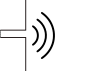
\includegraphics[width=0.55\textwidth]{lips_b}%
        \end{column}
    \end{columns}
        \begin{flalign*}
            & \mathcal{P}_N(l_N, z) = Z_L \mathcal{U}_N(l_N, z) &&
        \end{flalign*}
\end{frame}

\begin{frame}[t]{Сигнал от реч - модел на тръбите}
    \begin{columns}[T]
        \begin{column}{0.48\textwidth}
            {\tiny \begin{flalign*}
                & u_k(x, t) = \Q{u_k^+\B{t - \frac{x}{c}} - u_k^-\B{t + \frac{x}{c}}} && \\
                & p_k(x, t) = \cfrac{\rho c}{A_k}\Q{u_k^+\B{t - \frac{x}{c}} + u_k^-\B{t + \frac{x}{c}}} &&\\
                & U_k^{+}(z) = \cfrac{ z^{1/2}}{1 + r_k} U_{k+1}^{+}(z) - \cfrac{r_k z^{1/2}}{1+r_k} U_{k+1}^{-}(z) && \\
                & U_k^{-}(z) = - \cfrac{r_k z^{-1/2} }{1+r_k} U_{k+1}^{+}(z) + \cfrac{ z^{-1/2} }{1 + r_k} U_{k+1}^{-}(z)&&
            \end{flalign*}}
        \end{column}%
        \hfill%
        \begin{column}{0.24\textwidth}
        \end{column}%
        \hfill%
        \begin{column}{0.24\textwidth}
        \end{column}%
    \end{columns}
    \centering{Огрнаничения при устните}
    \begin{columns}[T]
        \begin{column}{0.48\textwidth}
            
\includegraphics[width=0.55\textwidth]{lips_a}%
        \end{column}
        \hfill
        \begin{column}{0.48\textwidth}
            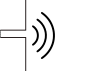
\includegraphics[width=0.55\textwidth]{lips_b}%
        \end{column}
    \end{columns}
        \begin{flalign*}
            & \mathcal{P}_N(l_N, z) = Z_L \mathcal{U}_N(l_N, z) \qquad p(l_N, t) \xleftrightarrow{\mathcal{F}\mathcal{S}}  \mathcal{P}_N(l_N, z), u_N(l_N, t) \xleftrightarrow{\mathcal{F}\mathcal{S}} \mathcal{U}_N(l_N, z)&&
        \end{flalign*}
\end{frame}

\begin{frame}[t]{Сигнал от реч - модел на тръбите}
    \begin{columns}[T]
        \begin{column}{0.48\textwidth}
            {\tiny \begin{flalign*}
                & {\color{mypink} u_k(x, t) = \Q{u_k^+\B{t - \frac{x}{c}} - u_k^-\B{t + \frac{x}{c}}}} && \\
                & {\color{mypink} p_k(x, t) = \cfrac{\rho c}{A_k}\Q{u_k^+\B{t - \frac{x}{c}} + u_k^-\B{t + \frac{x}{c}}}} &&\\
                & U_k^{+}(z) = \cfrac{ z^{1/2}}{1 + r_k} U_{k+1}^{+}(z) - \cfrac{r_k z^{1/2}}{1+r_k} U_{k+1}^{-}(z) && \\
                & U_k^{-}(z) = - \cfrac{r_k z^{-1/2} }{1+r_k} U_{k+1}^{+}(z) + \cfrac{ z^{-1/2} }{1 + r_k} U_{k+1}^{-}(z)&&
            \end{flalign*}}
        \end{column}%
        \hfill%
        \begin{column}{0.24\textwidth}
        \end{column}%
        \hfill%
        \begin{column}{0.24\textwidth}
        \end{column}%
    \end{columns}
    \centering{Огрнаничения при устните}
    \begin{columns}[T]
        \begin{column}{0.48\textwidth}
            
\includegraphics[width=0.55\textwidth]{lips_a}%
        \end{column}
        \hfill
        \begin{column}{0.48\textwidth}
            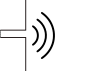
\includegraphics[width=0.55\textwidth]{lips_b}%
        \end{column}
    \end{columns}
        \begin{flalign*}
            & p_N(l_N, t) = Z_L u_N(l_N, t) &&
        \end{flalign*}
\end{frame}

\begin{frame}[t]{Сигнал от реч - модел на тръбите}
    \begin{columns}[T]
        \begin{column}{0.48\textwidth}
            {\tiny \begin{flalign*}
                & {\color{mypink} u_k(x, t) = \Q{u_k^+\B{t - \frac{x}{c}} - u_k^-\B{t + \frac{x}{c}}}} && \\
                & {\color{mypink} p_k(x, t) = \cfrac{\rho c}{A_k}\Q{u_k^+\B{t - \frac{x}{c}} + u_k^-\B{t + \frac{x}{c}}}} &&\\
                & U_k^{+}(z) = \cfrac{ z^{1/2}}{1 + r_k} U_{k+1}^{+}(z) - \cfrac{r_k z^{1/2}}{1+r_k} U_{k+1}^{-}(z) && \\
                & U_k^{-}(z) = - \cfrac{r_k z^{-1/2} }{1+r_k} U_{k+1}^{+}(z) + \cfrac{ z^{-1/2} }{1 + r_k} U_{k+1}^{-}(z)&&
            \end{flalign*}}
        \end{column}%
        \hfill%
        \begin{column}{0.24\textwidth}
        \end{column}%
        \hfill%
        \begin{column}{0.24\textwidth}
        \end{column}%
    \end{columns}
    \centering{Огрнаничения при устните}
    \begin{columns}[T]
        \begin{column}{0.48\textwidth}
            
\includegraphics[width=0.55\textwidth]{lips_a}%
        \end{column}
        \hfill
        \begin{column}{0.48\textwidth}
            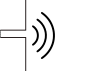
\includegraphics[width=0.55\textwidth]{lips_b}%
        \end{column}
    \end{columns}
        \begin{flalign*}
            & p_N(l_N, t) = Z_L u_N(l_N, t) &&\\
            &  u_N^{-}(t + \tau_N) \cfrac{(\rho c + A_N Z_L)}{A_N} = u_N^{+}(t - \tau_N) \cfrac{(A_N Z_L - \rho c)}{A_N} &&
        \end{flalign*}
\end{frame}

\begin{frame}[t]{Сигнал от реч - модел на тръбите}
    \begin{columns}[T]
        \begin{column}{0.48\textwidth}
            {\tiny \begin{flalign*}
                & {\color{mypink} u_k(x, t) = \Q{u_k^+\B{t - \frac{x}{c}} - u_k^-\B{t + \frac{x}{c}}}} && \\
                & {\color{mypink} p_k(x, t) = \cfrac{\rho c}{A_k}\Q{u_k^+\B{t - \frac{x}{c}} + u_k^-\B{t + \frac{x}{c}}}} &&\\
                & U_k^{+}(z) = \cfrac{ z^{1/2}}{1 + r_k} U_{k+1}^{+}(z) - \cfrac{r_k z^{1/2}}{1+r_k} U_{k+1}^{-}(z) && \\
                & U_k^{-}(z) = - \cfrac{r_k z^{-1/2} }{1+r_k} U_{k+1}^{+}(z) + \cfrac{ z^{-1/2} }{1 + r_k} U_{k+1}^{-}(z)&&
            \end{flalign*}}
        \end{column}%
        \hfill%
        \begin{column}{0.24\textwidth}
        \end{column}%
        \hfill%
        \begin{column}{0.24\textwidth}
        \end{column}%
    \end{columns}
    \centering{Огрнаничения при устните}
    \begin{columns}[T]
        \begin{column}{0.48\textwidth}
            
\includegraphics[width=0.55\textwidth]{lips_a}%
        \end{column}
        \hfill
        \begin{column}{0.48\textwidth}
            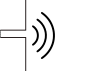
\includegraphics[width=0.55\textwidth]{lips_b}%
        \end{column}
    \end{columns}
        \begin{flalign*}
            & p_N(l_N, t) = Z_L u_N(l_N, t) &&\\
            &  u_N^{-}(t + \tau_N) \cfrac{(\rho c + A_N Z_L)}{A_N} = u_N^{+}(t - \tau_N) \cfrac{(A_N Z_L - \rho c)}{A_N} \qquad r_L = \cfrac{\frac{\rho c}{Z_L} - A_N}{\frac{\rho c}{Z_L} + A_N}&&
        \end{flalign*}
\end{frame}

\begin{frame}[t]{Сигнал от реч - модел на тръбите}
    \begin{columns}[T]
        \begin{column}{0.48\textwidth}
            {\tiny \begin{flalign*}
                & {\color{mypink} u_k(x, t) = \Q{u_k^+\B{t - \frac{x}{c}} - u_k^-\B{t + \frac{x}{c}}}} && \\
                & {\color{mypink} p_k(x, t) = \cfrac{\rho c}{A_k}\Q{u_k^+\B{t - \frac{x}{c}} + u_k^-\B{t + \frac{x}{c}}}} &&\\
                & U_k^{+}(z) = \cfrac{ z^{1/2}}{1 + r_k} U_{k+1}^{+}(z) - \cfrac{r_k z^{1/2}}{1+r_k} U_{k+1}^{-}(z) && \\
                & U_k^{-}(z) = - \cfrac{r_k z^{-1/2} }{1+r_k} U_{k+1}^{+}(z) + \cfrac{ z^{-1/2} }{1 + r_k} U_{k+1}^{-}(z)&&
            \end{flalign*}}
        \end{column}%
        \hfill%
        \begin{column}{0.24\textwidth}
        \end{column}%
        \hfill%
        \begin{column}{0.24\textwidth}
        \end{column}%
    \end{columns}
    \centering{Огрнаничения при устните}
    \begin{columns}[T]
        \begin{column}{0.48\textwidth}
            
\includegraphics[width=0.55\textwidth]{lips_a}%
        \end{column}
        \hfill
        \begin{column}{0.48\textwidth}
            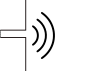
\includegraphics[width=0.55\textwidth]{lips_b}%
        \end{column}
    \end{columns}
        \begin{flalign*}
            & p_N(l_N, t) = Z_L u_N(l_N, t) &&\\
            &  u_N^{-}(t + \tau_N) = -r_L u_N^{+}(t - \tau_N) \qquad r_L = \cfrac{\frac{\rho c}{Z_L} - A_N}{\frac{\rho c}{Z_L} + A_N}&&
        \end{flalign*}
\end{frame}

\begin{frame}[t]{Сигнал от реч - модел на тръбите}
    \begin{columns}[T]
        \begin{column}{0.48\textwidth}
            {\tiny \begin{flalign*}
                & {\color{mypink} u_k(x, t) = \Q{u_k^+\B{t - \frac{x}{c}} - u_k^-\B{t + \frac{x}{c}}}} && \\
                & {\color{mypink} p_k(x, t) = \cfrac{\rho c}{A_k}\Q{u_k^+\B{t - \frac{x}{c}} + u_k^-\B{t + \frac{x}{c}}}} &&\\
                & U_k^{+}(z) = \cfrac{ z^{1/2}}{1 + r_k} U_{k+1}^{+}(z) - \cfrac{r_k z^{1/2}}{1+r_k} U_{k+1}^{-}(z) && \\
                & U_k^{-}(z) = - \cfrac{r_k z^{-1/2} }{1+r_k} U_{k+1}^{+}(z) + \cfrac{ z^{-1/2} }{1 + r_k} U_{k+1}^{-}(z)&&
            \end{flalign*}}
        \end{column}%
        \hfill%
        \begin{column}{0.24\textwidth}
            {\tiny \begin{flalign*}
                & r_L = \cfrac{\frac{\rho c}{Z_L} - A_N}{\frac{\rho c}{Z_L} + A_N} &&
            \end{flalign*}}
        \end{column}%
        \hfill%
        \begin{column}{0.24\textwidth}
        \end{column}%
    \end{columns}
    \centering{Огрнаничения при устните}
    \begin{columns}[T]
        \begin{column}{0.48\textwidth}
            
\includegraphics[width=0.55\textwidth]{lips_a}%
        \end{column}
        \hfill
        \begin{column}{0.48\textwidth}
            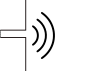
\includegraphics[width=0.55\textwidth]{lips_b}%
        \end{column}
    \end{columns}
    \begin{flalign*}
        & p_N(l_N, t) = Z_L u_N(l_N, t) &&\\
        &  u_N^{-}(t + \tau_N) = -r_L u_N^{+}(t - \tau_N) \qquad r_L = \cfrac{\frac{\rho c}{Z_L} - A_N}{\frac{\rho c}{Z_L} + A_N}&&
    \end{flalign*}
\end{frame}

\begin{frame}[t]{Сигнал от реч - модел на тръбите}
    \begin{columns}[T]
        \begin{column}{0.48\textwidth}
            {\tiny \begin{flalign*}
                & u_k(x, t) = \Q{u_k^+\B{t - \frac{x}{c}} - u_k^-\B{t + \frac{x}{c}}} && \\
                & p_k(x, t) = \cfrac{\rho c}{A_k}\Q{u_k^+\B{t - \frac{x}{c}} + u_k^-\B{t + \frac{x}{c}}} &&\\
                & U_k^{+}(z) = \cfrac{ z^{1/2}}{1 + r_k} U_{k+1}^{+}(z) - \cfrac{r_k z^{1/2}}{1+r_k} U_{k+1}^{-}(z) && \\
                & U_k^{-}(z) = - \cfrac{r_k z^{-1/2} }{1+r_k} U_{k+1}^{+}(z) + \cfrac{ z^{-1/2} }{1 + r_k} U_{k+1}^{-}(z)&&
            \end{flalign*}}
        \end{column}%
        \hfill%
        \begin{column}{0.14\textwidth}
            {\tiny \begin{flalign*}
                & r_L = \cfrac{\frac{\rho c}{Z_L} - A_N}{\frac{\rho c}{Z_L} + A_N} &&
            \end{flalign*}}
        \end{column}%
        \hfill%
        \begin{column}{0.34\textwidth}
        \end{column}%
    \end{columns}
    \pause
    \centering{Огрнаничения при глотиса}
    \pause
    {\small \begin{flalign*}
        & U_1(0, z) =  U_G(z) - \frac{P_1(0, z)}{Z_G(z)} &&\\
    \end{flalign*}}
\end{frame}

\begin{frame}[t]{Сигнал от реч - модел на тръбите}
    \begin{columns}[T]
        \begin{column}{0.48\textwidth}
            {\tiny \begin{flalign*}
                & u_k(x, t) = \Q{u_k^+\B{t - \frac{x}{c}} - u_k^-\B{t + \frac{x}{c}}} && \\
                & p_k(x, t) = \cfrac{\rho c}{A_k}\Q{u_k^+\B{t - \frac{x}{c}} + u_k^-\B{t + \frac{x}{c}}} &&\\
                & U_k^{+}(z) = \cfrac{ z^{1/2}}{1 + r_k} U_{k+1}^{+}(z) - \cfrac{r_k z^{1/2}}{1+r_k} U_{k+1}^{-}(z) && \\
                & U_k^{-}(z) = - \cfrac{r_k z^{-1/2} }{1+r_k} U_{k+1}^{+}(z) + \cfrac{ z^{-1/2} }{1 + r_k} U_{k+1}^{-}(z)&&
            \end{flalign*}}
        \end{column}%
        \hfill%
        \begin{column}{0.14\textwidth}
            {\tiny \begin{flalign*}
                & r_L = \cfrac{\frac{\rho c}{Z_L} - A_N}{\frac{\rho c}{Z_L} + A_N} &&
            \end{flalign*}}
        \end{column}%
        \hfill%
        \begin{column}{0.34\textwidth}
        \end{column}%
    \end{columns}
    \centering{Огрнаничения при глотиса}
    {\small \begin{flalign*}
        & U_1(0, z) =  U_G(z) - \frac{P_1(0, z)}{Z_G} &&\\
    \end{flalign*}}
\end{frame}

\begin{frame}[t]{Сигнал от реч - модел на тръбите}
    \begin{columns}[T]
        \begin{column}{0.48\textwidth}
            {\tiny \begin{flalign*}
                & u_k(x, t) = \Q{u_k^+\B{t - \frac{x}{c}} - u_k^-\B{t + \frac{x}{c}}} && \\
                & p_k(x, t) = \cfrac{\rho c}{A_k}\Q{u_k^+\B{t - \frac{x}{c}} + u_k^-\B{t + \frac{x}{c}}} &&\\
                & U_k^{+}(z) = \cfrac{ z^{1/2}}{1 + r_k} U_{k+1}^{+}(z) - \cfrac{r_k z^{1/2}}{1+r_k} U_{k+1}^{-}(z) && \\
                & U_k^{-}(z) = - \cfrac{r_k z^{-1/2} }{1+r_k} U_{k+1}^{+}(z) + \cfrac{ z^{-1/2} }{1 + r_k} U_{k+1}^{-}(z)&&
            \end{flalign*}}
        \end{column}%
        \hfill%
        \begin{column}{0.14\textwidth}
            {\tiny \begin{flalign*}
                & r_L = \cfrac{\frac{\rho c}{Z_L} - A_N}{\frac{\rho c}{Z_L} + A_N} &&
            \end{flalign*}}
        \end{column}%
        \hfill%
        \begin{column}{0.34\textwidth}
        \end{column}%
    \end{columns}
    \centering{Огрнаничения при глотиса}
    {\small \begin{flalign*}
        & U_1(0, z) =  U_G(z) - \frac{P_1(0, z)}{Z_G} && \\
        & u_1(0, t) \xleftrightarrow{\mathcal{F}\mathcal{S}} U_1(0, z), u_G(t) \xleftrightarrow{\mathcal{F}\mathcal{S}} U_G(z), p_1(0, t) \xleftrightarrow{\mathcal{F}\mathcal{S}} P_1(0, z) &&\\
    \end{flalign*}}
\end{frame}

\begin{frame}[t]{Сигнал от реч - модел на тръбите}
    \begin{columns}[T]
        \begin{column}{0.48\textwidth}
            {\tiny \begin{flalign*}
                & u_k(x, t) = \Q{u_k^+\B{t - \frac{x}{c}} - u_k^-\B{t + \frac{x}{c}}} && \\
                & p_k(x, t) = \cfrac{\rho c}{A_k}\Q{u_k^+\B{t - \frac{x}{c}} + u_k^-\B{t + \frac{x}{c}}} &&\\
                & U_k^{+}(z) = \cfrac{ z^{1/2}}{1 + r_k} U_{k+1}^{+}(z) - \cfrac{r_k z^{1/2}}{1+r_k} U_{k+1}^{-}(z) && \\
                & U_k^{-}(z) = - \cfrac{r_k z^{-1/2} }{1+r_k} U_{k+1}^{+}(z) + \cfrac{ z^{-1/2} }{1 + r_k} U_{k+1}^{-}(z)&&
            \end{flalign*}}
        \end{column}%
        \hfill%
        \begin{column}{0.14\textwidth}
            {\tiny \begin{flalign*}
                & r_L = \cfrac{\frac{\rho c}{Z_L} - A_N}{\frac{\rho c}{Z_L} + A_N} &&
            \end{flalign*}}
        \end{column}%
        \hfill%
        \begin{column}{0.34\textwidth}
        \end{column}%
    \end{columns}
    \centering{Огрнаничения при глотиса}
    {\small \begin{flalign*}
        & U_1(0, z) =  U_G(z) - \frac{P_1(0, z)}{Z_G} && \\
        & u_1(0, t) \xleftrightarrow{\mathcal{F}\mathcal{S}} U_1(0, z), u_G(t) \xleftrightarrow{\mathcal{F}\mathcal{S}} U_G(z), p_1(0, t) \xleftrightarrow{\mathcal{F}\mathcal{S}} P_1(0, z) &&\\
        & u_1(0, t) = u_G(t) - \frac{p_1(0, t)}{Z_G}&&
    \end{flalign*}}
\end{frame}

\begin{frame}[t]{Сигнал от реч - модел на тръбите}
    \begin{columns}[T]
        \begin{column}{0.48\textwidth}
            {\tiny \begin{flalign*}
                & {\color{mypink} u_k(x, t) = \Q{u_k^+\B{t - \frac{x}{c}} - u_k^-\B{t + \frac{x}{c}}}} && \\
                & {\color{mypink} p_k(x, t) = \cfrac{\rho c}{A_k}\Q{u_k^+\B{t - \frac{x}{c}} + u_k^-\B{t + \frac{x}{c}}}} &&\\
                & U_k^{+}(z) = \cfrac{ z^{1/2}}{1 + r_k} U_{k+1}^{+}(z) - \cfrac{r_k z^{1/2}}{1+r_k} U_{k+1}^{-}(z) && \\
                & U_k^{-}(z) = - \cfrac{r_k z^{-1/2} }{1+r_k} U_{k+1}^{+}(z) + \cfrac{ z^{-1/2} }{1 + r_k} U_{k+1}^{-}(z)&&
            \end{flalign*}}
        \end{column}%
        \hfill%
        \begin{column}{0.14\textwidth}
            {\tiny \begin{flalign*}
                & r_L = \cfrac{\frac{\rho c}{Z_L} - A_N}{\frac{\rho c}{Z_L} + A_N} &&
            \end{flalign*}}
        \end{column}%
        \hfill%
        \begin{column}{0.34\textwidth}
        \end{column}%
    \end{columns}
    \centering{Огрнаничения при глотиса}
    {\small \begin{flalign*}
        & U_1(0, z) =  U_G(z) - \frac{P_1(0, z)}{Z_G} && \\
        & u_1(0, t) \xleftrightarrow{\mathcal{F}\mathcal{S}} U_1(0, z), u_G(t) \xleftrightarrow{\mathcal{F}\mathcal{S}} U_G(z), p_1(0, t) \xleftrightarrow{\mathcal{F}\mathcal{S}} P_1(0, z) &&\\
        & u_1(0, t) = u_G(t) - \frac{p_1(0, t)}{Z_G}&&
    \end{flalign*}}
\end{frame}


\begin{frame}[t]{Сигнал от реч - модел на тръбите}
    \begin{columns}[T]
        \begin{column}{0.48\textwidth}
            {\tiny \begin{flalign*}
                & {\color{mypink} u_k(x, t) = \Q{u_k^+\B{t - \frac{x}{c}} - u_k^-\B{t + \frac{x}{c}}}} && \\
                & {\color{mypink} p_k(x, t) = \cfrac{\rho c}{A_k}\Q{u_k^+\B{t - \frac{x}{c}} + u_k^-\B{t + \frac{x}{c}}}} &&\\
                & U_k^{+}(z) = \cfrac{ z^{1/2}}{1 + r_k} U_{k+1}^{+}(z) - \cfrac{r_k z^{1/2}}{1+r_k} U_{k+1}^{-}(z) && \\
                & U_k^{-}(z) = - \cfrac{r_k z^{-1/2} }{1+r_k} U_{k+1}^{+}(z) + \cfrac{ z^{-1/2} }{1 + r_k} U_{k+1}^{-}(z)&&
            \end{flalign*}}
        \end{column}%
        \hfill%
        \begin{column}{0.14\textwidth}
            {\tiny \begin{flalign*}
                & r_L = \cfrac{\frac{\rho c}{Z_L} - A_N}{\frac{\rho c}{Z_L} + A_N} &&
            \end{flalign*}}
        \end{column}%
        \hfill%
        \begin{column}{0.34\textwidth}
        \end{column}%
    \end{columns}
    \centering{Огрнаничения при глотиса}
    {\small \begin{flalign*}
        & U_1(0, z) =  U_G(z) - \frac{P_1(0, z)}{Z_G} && \\
        & u_1(0, t) \xleftrightarrow{\mathcal{F}\mathcal{S}} U_1(0, z), u_G(t) \xleftrightarrow{\mathcal{F}\mathcal{S}} U_G(z), p_1(0, t) \xleftrightarrow{\mathcal{F}\mathcal{S}} P_1(0, z) &&\\
        & u_1(0, t) = u_G(t) - \frac{p_1(0, t)}{Z_G}&& \\
        & u_1^{+}(t) = u_G(t)\Q{\frac{A_1 Z_G}{A_1 Z_G + \rho  c}} + u_1^{-}(t)\Q{\frac{A_1 Z_G - \rho  c}{A_1 Z_G + \rho  c}} &&
    \end{flalign*}}
\end{frame}

\begin{frame}[t]{Сигнал от реч - модел на тръбите}
    \begin{columns}[T]
        \begin{column}{0.48\textwidth}
            {\tiny \begin{flalign*}
                & u_k(x, t) = \Q{u_k^+\B{t - \frac{x}{c}} - u_k^-\B{t + \frac{x}{c}}} && \\
                & p_k(x, t) = \cfrac{\rho c}{A_k}\Q{u_k^+\B{t - \frac{x}{c}} + u_k^-\B{t + \frac{x}{c}}} &&\\
                & U_k^{+}(z) = \cfrac{ z^{1/2}}{1 + r_k} U_{k+1}^{+}(z) - \cfrac{r_k z^{1/2}}{1+r_k} U_{k+1}^{-}(z) && \\
                & U_k^{-}(z) = - \cfrac{r_k z^{-1/2} }{1+r_k} U_{k+1}^{+}(z) + \cfrac{ z^{-1/2} }{1 + r_k} U_{k+1}^{-}(z)&&
            \end{flalign*}}
        \end{column}%
        \hfill%
        \begin{column}{0.14\textwidth}
            {\tiny \begin{flalign*}
                & r_L = \cfrac{\frac{\rho c}{Z_L} - A_N}{\frac{\rho c}{Z_L} + A_N} &&
            \end{flalign*}}
        \end{column}%
        \hfill%
        \begin{column}{0.34\textwidth}
        \end{column}%
    \end{columns}
    \centering{Огрнаничения при глотиса}
    {\small \begin{flalign*}
        & U_1(0, z) =  U_G(z) - \frac{P_1(0, z)}{Z_G} && \\
        & u_1(0, t) \xleftrightarrow{\mathcal{F}\mathcal{S}} U_1(0, z), u_G(t) \xleftrightarrow{\mathcal{F}\mathcal{S}} U_G(z), p_1(0, t) \xleftrightarrow{\mathcal{F}\mathcal{S}} P_1(0, z) &&\\
        & u_1(0, t) = u_G(t) - \frac{p_1(0, t)}{Z_G}&& \\
        & u_1^{+}(t) = u_G(t)\Q{\frac{A_1 Z_G}{A_1 Z_G + \rho  c}} + u_1^{-}(t)\Q{\frac{A_1 Z_G - \rho  c}{A_1 Z_G + \rho  c}} \qquad r_G = \B{\cfrac{A_1 Z_G - \rho c}{A_1 Z_G + \rho c}}&&
    \end{flalign*}}
\end{frame}


\begin{frame}[t]{Сигнал от реч - модел на тръбите}
    \begin{columns}[T]
        \begin{column}{0.48\textwidth}
            {\tiny \begin{flalign*}
                & u_k(x, t) = \Q{u_k^+\B{t - \frac{x}{c}} - u_k^-\B{t + \frac{x}{c}}} && \\
                & p_k(x, t) = \cfrac{\rho c}{A_k}\Q{u_k^+\B{t - \frac{x}{c}} + u_k^-\B{t + \frac{x}{c}}} &&\\
                & U_k^{+}(z) = \cfrac{ z^{1/2}}{1 + r_k} U_{k+1}^{+}(z) - \cfrac{r_k z^{1/2}}{1+r_k} U_{k+1}^{-}(z) && \\
                & U_k^{-}(z) = - \cfrac{r_k z^{-1/2} }{1+r_k} U_{k+1}^{+}(z) + \cfrac{ z^{-1/2} }{1 + r_k} U_{k+1}^{-}(z)&&
            \end{flalign*}}
        \end{column}%
        \hfill%
        \begin{column}{0.14\textwidth}
            {\tiny \begin{flalign*}
                & r_L = \cfrac{\frac{\rho c}{Z_L} - A_N}{\frac{\rho c}{Z_L} + A_N} &&
            \end{flalign*}}
        \end{column}%
        \hfill%
        \begin{column}{0.34\textwidth}
        \end{column}%
    \end{columns}
    \centering{Огрнаничения при глотиса}
    {\small \begin{flalign*}
        & U_1(0, z) =  U_G(z) - \frac{P_1(0, z)}{Z_G} && \\
        & u_1(0, t) \xleftrightarrow{\mathcal{F}\mathcal{S}} U_1(0, z), u_G(t) \xleftrightarrow{\mathcal{F}\mathcal{S}} U_G(z), p_1(0, t) \xleftrightarrow{\mathcal{F}\mathcal{S}} P_1(0, z) &&\\
        & u_1(0, t) = u_G(t) - \frac{p_1(0, t)}{Z_G}&& \\
        & u_1^{+}(t) = u_G(t) \Q{\frac{1 + r_G}{2}} + r_G u_1^{-}(t) \qquad r_G = \B{\cfrac{A_1 Z_G - \rho c}{A_1 Z_G + \rho c}}&&
    \end{flalign*}}
\end{frame}

\begin{frame}[t]{Сигнал от реч - модел на тръбите}
    \begin{columns}[T]
        \begin{column}{0.48\textwidth}
            {\tiny \begin{flalign*}
                & u_k(x, t) = \Q{u_k^+\B{t - \frac{x}{c}} - u_k^-\B{t + \frac{x}{c}}} && \\
                & p_k(x, t) = \cfrac{\rho c}{A_k}\Q{u_k^+\B{t - \frac{x}{c}} + u_k^-\B{t + \frac{x}{c}}} &&\\
                & U_k^{+}(z) = \cfrac{ z^{1/2}}{1 + r_k} U_{k+1}^{+}(z) - \cfrac{r_k z^{1/2}}{1+r_k} U_{k+1}^{-}(z) && \\
                & U_k^{-}(z) = - \cfrac{r_k z^{-1/2} }{1+r_k} U_{k+1}^{+}(z) + \cfrac{ z^{-1/2} }{1 + r_k} U_{k+1}^{-}(z)&&
            \end{flalign*}}
        \end{column}%
        \hfill%
        \begin{column}{0.14\textwidth}
            {\tiny \begin{flalign*}
                & r_L = \cfrac{\frac{\rho c}{Z_L} - A_N}{\frac{\rho c}{Z_L} + A_N} &&
            \end{flalign*}}
        \end{column}%
        \hfill%
        \begin{column}{0.34\textwidth}
        \end{column}%
    \end{columns}
    \centering{Огрнаничения при глотиса}
    {\small \begin{flalign*}
        & U_1(0, z) =  U_G(z) - \frac{P_1(0, z)}{Z_G} && \\
        & u_1(0, t) \xleftrightarrow{\mathcal{F}\mathcal{S}} U_1(0, z), u_G(t) \xleftrightarrow{\mathcal{F}\mathcal{S}} U_G(z), p_1(0, t) \xleftrightarrow{\mathcal{F}\mathcal{S}} P_1(0, z) &&\\
        & u_1(0, t) = u_G(t) - \frac{p_1(0, t)}{Z_G}&& \\
        & u_1^{+}(t) = u_G(t) \Q{\frac{1 + r_G}{2}} + r_G u_1^{-}(t) \qquad r_G = \B{\cfrac{A_1 Z_G - \rho c}{A_1 Z_G + \rho c}}&&\\
        & U_1^{+}(z) = U_G(z) \Q{\frac{1 + r_G}{2}} + r_G U_1^{-}(z) &&
    \end{flalign*}}
\end{frame}

\begin{frame}[t]{Сигнал от реч - модел на тръбите}
    \begin{columns}[T]
        \begin{column}{0.48\textwidth}
            {\tiny \begin{flalign*}
                & u_k(x, t) = \Q{u_k^+\B{t - \frac{x}{c}} - u_k^-\B{t + \frac{x}{c}}} && \\
                & p_k(x, t) = \cfrac{\rho c}{A_k}\Q{u_k^+\B{t - \frac{x}{c}} + u_k^-\B{t + \frac{x}{c}}} &&\\
                & U_k^{+}(z) = \cfrac{ z^{1/2}}{1 + r_k} U_{k+1}^{+}(z) - \cfrac{r_k z^{1/2}}{1+r_k} U_{k+1}^{-}(z) && \\
                & U_k^{-}(z) = - \cfrac{r_k z^{-1/2} }{1+r_k} U_{k+1}^{+}(z) + \cfrac{ z^{-1/2} }{1 + r_k} U_{k+1}^{-}(z)&&
            \end{flalign*}}
        \end{column}%
        \hfill%
        \begin{column}{0.14\textwidth}
            {\tiny \begin{flalign*}
                & r_L = \cfrac{\frac{\rho c}{Z_L} - A_N}{\frac{\rho c}{Z_L} + A_N} &&
            \end{flalign*}}
        \end{column}%
        \hfill%
        \begin{column}{0.34\textwidth}
            {\tiny \begin{flalign*}
                & r_G = \B{\cfrac{A_1 Z_G - \rho c}{A_1 Z_G + \rho c}} &&\\
                & U_1^{+}(z) = U_G(z) \Q{\frac{1 + r_G}{2}} + r_G U_1^{-}(z) &&
            \end{flalign*}}
        \end{column}%
    \end{columns}
    \centering{Огрнаничения при глотиса}
    {\small \begin{flalign*}
        & U_1(0, z) =  U_G(z) - \frac{P_1(0, z)}{Z_G} && \\
        & u_1(0, t) \xleftrightarrow{\mathcal{F}\mathcal{S}} U_1(0, z), u_G(t) \xleftrightarrow{\mathcal{F}\mathcal{S}} U_G(z), p_1(0, t) \xleftrightarrow{\mathcal{F}\mathcal{S}} P_1(0, z) &&\\
        & u_1(0, t) = u_G(t) - \frac{p_1(0, t)}{Z_G}&& \\
        & u_1^{+}(t) = u_G(t) \Q{\frac{1 + r_G}{2}} + r_G u_1^{-}(t) \qquad r_G = \B{\cfrac{A_1 Z_G - \rho c}{A_1 Z_G + \rho c}}&&\\
        & U_1^{+}(z) = U_G(z) \Q{\frac{1 + r_G}{2}} + r_G U_1^{-}(z) &&
    \end{flalign*}}
\end{frame}

\begin{frame}[t]{Сигнал от реч - модел на тръбите}
    \begin{columns}[T]
        \begin{column}{0.48\textwidth}
            {\tiny \begin{flalign*}
                & u_k(x, t) = \Q{u_k^+\B{t - \frac{x}{c}} - u_k^-\B{t + \frac{x}{c}}} && \\
                & p_k(x, t) = \cfrac{\rho c}{A_k}\Q{u_k^+\B{t - \frac{x}{c}} + u_k^-\B{t + \frac{x}{c}}} &&\\
                & U_k^{+}(z) = \cfrac{ z^{1/2}}{1 + r_k} U_{k+1}^{+}(z) - \cfrac{r_k z^{1/2}}{1+r_k} U_{k+1}^{-}(z) && \\
                & U_k^{-}(z) = - \cfrac{r_k z^{-1/2} }{1+r_k} U_{k+1}^{+}(z) + \cfrac{ z^{-1/2} }{1 + r_k} U_{k+1}^{-}(z)&&
            \end{flalign*}}
        \end{column}%
        \hfill%
        \begin{column}{0.14\textwidth}
            {\tiny \begin{flalign*}
                & r_L = \cfrac{\frac{\rho c}{Z_L} - A_N}{\frac{\rho c}{Z_L} + A_N} &&
            \end{flalign*}}
        \end{column}%
        \hfill%
        \begin{column}{0.34\textwidth}
            {\tiny \begin{flalign*}
                & r_G = \B{\cfrac{A_1 Z_G - \rho c}{A_1 Z_G + \rho c}} &&\\
                & U_1^{+}(z) = U_G(z) \Q{\frac{1 + r_G}{2}} + r_G U_1^{-}(z) &&
            \end{flalign*}}
        \end{column}%
    \end{columns}
\end{frame}

\begin{frame}[t]{Сигнал от реч - модел на тръбите}
    \begin{columns}[T]
        \begin{column}{0.48\textwidth}
            {\tiny \begin{flalign*}
                & U_k^{+}(z) = \cfrac{ z^{1/2}}{1 + r_k} U_{k+1}^{+}(z) - \cfrac{r_k z^{1/2}}{1+r_k} U_{k+1}^{-}(z) && \\
                & U_k^{-}(z) = - \cfrac{r_k z^{-1/2} }{1+r_k} U_{k+1}^{+}(z) + \cfrac{ z^{-1/2} }{1 + r_k} U_{k+1}^{-}(z)&&
            \end{flalign*}}
        \end{column}%
        \hfill%
        \begin{column}{0.14\textwidth}
            {\tiny \begin{flalign*}
                & r_L = \cfrac{\frac{\rho c}{Z_L} - A_N}{\frac{\rho c}{Z_L} + A_N} &&
            \end{flalign*}}
        \end{column}%
        \hfill%
        \begin{column}{0.34\textwidth}
            {\tiny \begin{flalign*}
                & r_G = \B{\cfrac{A_1 Z_G - \rho c}{A_1 Z_G + \rho c}} &&\\
                & U_1^{+}(z) = U_G(z) \Q{\frac{1 + r_G}{2}} + r_G U_1^{-}(z) &&
            \end{flalign*}}
        \end{column}%
    \end{columns}
    \pause
    \centering{Общ вид}
    \pause
    \begin{flalign*}
            & U_{N+1}^{+} (z) = U_L(z) &&
    \end{flalign*}
\end{frame}

\begin{frame}[t]{Сигнал от реч - модел на тръбите}
    \begin{columns}[T]
        \begin{column}{0.48\textwidth}
            {\tiny \begin{flalign*}
                & U_k^{+}(z) = \cfrac{ z^{1/2}}{1 + r_k} U_{k+1}^{+}(z) - \cfrac{r_k z^{1/2}}{1+r_k} U_{k+1}^{-}(z) && \\
                & U_k^{-}(z) = - \cfrac{r_k z^{-1/2} }{1+r_k} U_{k+1}^{+}(z) + \cfrac{ z^{-1/2} }{1 + r_k} U_{k+1}^{-}(z)&&
            \end{flalign*}}
        \end{column}%
        \hfill%
        \begin{column}{0.14\textwidth}
            {\tiny \begin{flalign*}
                & r_L = \cfrac{\frac{\rho c}{Z_L} - A_N}{\frac{\rho c}{Z_L} + A_N} &&
            \end{flalign*}}
        \end{column}%
        \hfill%
        \begin{column}{0.34\textwidth}
            {\tiny \begin{flalign*}
                & r_G = \B{\cfrac{A_1 Z_G - \rho c}{A_1 Z_G + \rho c}} &&\\
                & U_1^{+}(z) = U_G(z) \Q{\frac{1 + r_G}{2}} + r_G U_1^{-}(z) &&
            \end{flalign*}}
        \end{column}%
    \end{columns}
    \centering{Общ вид}
    \begin{flalign*}
        & U_{N+1}^{+} (z) = U_L(z) &&\\
        & U_{N+1}^{-}(z) = 0 &&
    \end{flalign*}
\end{frame}

\begin{frame}[t]{Сигнал от реч - модел на тръбите}
    \begin{columns}[T]
        \begin{column}{0.48\textwidth}
            {\tiny \begin{flalign*}
                & U_k^{+}(z) = \cfrac{ z^{1/2}}{1 + r_k} U_{k+1}^{+}(z) - \cfrac{r_k z^{1/2}}{1+r_k} U_{k+1}^{-}(z) && \\
                & U_k^{-}(z) = - \cfrac{r_k z^{-1/2} }{1+r_k} U_{k+1}^{+}(z) + \cfrac{ z^{-1/2} }{1 + r_k} U_{k+1}^{-}(z)&&
            \end{flalign*}}
        \end{column}%
        \hfill%
        \begin{column}{0.14\textwidth}
            {\tiny \begin{flalign*}
                & r_L = \cfrac{\frac{\rho c}{Z_L} - A_N}{\frac{\rho c}{Z_L} + A_N} &&
            \end{flalign*}}
        \end{column}%
        \hfill%
        \begin{column}{0.34\textwidth}
            {\tiny \begin{flalign*}
                & r_G = \B{\cfrac{A_1 Z_G - \rho c}{A_1 Z_G + \rho c}} &&\\
                & U_1^{+}(z) = U_G(z) \Q{\frac{1 + r_G}{2}} + r_G U_1^{-}(z) &&
            \end{flalign*}}
        \end{column}%
    \end{columns}
    \centering{Общ вид}
    \begin{flalign*}
        & U_{N+1}^{+} (z) = U_L(z) &&\\
        & U_{N+1}^{-}(z) = 0 && \\
        & r_N = r_L &&
    \end{flalign*}
\end{frame}

\begin{frame}[t]{Сигнал от реч - модел на тръбите}
    \begin{columns}[T]
        \begin{column}{0.48\textwidth}
            {\tiny \begin{flalign*}
                & U_k^{+}(z) = \cfrac{ z^{1/2}}{1 + r_k} U_{k+1}^{+}(z) - \cfrac{r_k z^{1/2}}{1+r_k} U_{k+1}^{-}(z) && \\
                & U_k^{-}(z) = - \cfrac{r_k z^{-1/2} }{1+r_k} U_{k+1}^{+}(z) + \cfrac{ z^{-1/2} }{1 + r_k} U_{k+1}^{-}(z)&&
            \end{flalign*}}
        \end{column}%
        \hfill%
        \begin{column}{0.14\textwidth}
            {\tiny \begin{flalign*}
                & r_L = \cfrac{\frac{\rho c}{Z_L} - A_N}{\frac{\rho c}{Z_L} + A_N} &&
            \end{flalign*}}
        \end{column}%
        \hfill%
        \begin{column}{0.34\textwidth}
            {\tiny \begin{flalign*}
                & r_G = \B{\cfrac{A_1 Z_G - \rho c}{A_1 Z_G + \rho c}} &&\\
                & U_1^{+}(z) = U_G(z) \Q{\frac{1 + r_G}{2}} + r_G U_1^{-}(z) &&
            \end{flalign*}}
        \end{column}%
    \end{columns}
    \centering{Общ вид}
    \begin{flalign*}
        & U_{N+1}^{+} (z) = U_L(z) &&\\
        & U_{N+1}^{-}(z) = 0 && \\
        & r_N = r_L \rightarrow A_{N+1} = \cfrac{\rho c}{Z_L}&&
    \end{flalign*}
\end{frame}

\begin{frame}[t]{Сигнал от реч - модел на тръбите}
    \begin{columns}[T]
        \begin{column}{0.48\textwidth}
            {\tiny \begin{flalign*}
                & U_k^{+}(z) = \cfrac{ z^{1/2}}{1 + r_k} U_{k+1}^{+}(z) - \cfrac{r_k z^{1/2}}{1+r_k} U_{k+1}^{-}(z) && \\
                & U_k^{-}(z) = - \cfrac{r_k z^{-1/2} }{1+r_k} U_{k+1}^{+}(z) + \cfrac{ z^{-1/2} }{1 + r_k} U_{k+1}^{-}(z)&&
            \end{flalign*}}
        \end{column}%
        \hfill%
        \begin{column}{0.14\textwidth}
            {\tiny \begin{flalign*}
                & r_L = \cfrac{\frac{\rho c}{Z_L} - A_N}{\frac{\rho c}{Z_L} + A_N} &&
            \end{flalign*}}
        \end{column}%
        \hfill%
        \begin{column}{0.34\textwidth}
            {\tiny \begin{flalign*}
                & r_G = \B{\cfrac{A_1 Z_G - \rho c}{A_1 Z_G + \rho c}} &&\\
                & U_1^{+}(z) = U_G(z) \Q{\frac{1 + r_G}{2}} + r_G U_1^{-}(z) &&
            \end{flalign*}}
        \end{column}%
    \end{columns}
    \centering{Общ вид}
    \begin{flalign*}
        & U_{N+1}^{+} (z) = U_L(z) &&\\
        & U_{N+1}^{-}(z) = 0 && \\
        & r_N = r_L \rightarrow A_{N+1} = \cfrac{\rho c}{Z_L}&&
    \end{flalign*}
    $U_k = Q_k U_{k+1}$ за
    \begin{columns}[T]
        \begin{column}{0.48\textwidth}
            $U_k = 
            \begin{bmatrix}
                U_k^{+}(z) \\
                U_k^{-}(z) \\
            \end{bmatrix}$
        \end{column}
        \hfill
        \begin{column}{0.48\textwidth}
            $Q_k = 
            \begin{bmatrix}
                \cfrac{z^{1/2}}{1 + r_k} & \cfrac{-r_k z^{1/2}}{1 + r_k} \\
                & \\
                \cfrac{-r_k z^{-1/2}}{1 + r_k} & \cfrac{z^{-1/2}}{1 + r_k} \\
            \end{bmatrix}$
        \end{column}
    \end{columns}   
\end{frame}


\end{document}